%%%%%%%%%%%%%%%%%%%%%%%%%%%%%%%%%%%%%%%%%%%%%%%%%%%%%%%%%%%%%%%%%%%%%%%%%%%%%%%%
%% Plantilla de memoria en LaTeX para TFG/TFM - Universidad Rey Juan Carlos
%%
%% Por Gregorio Robles <grex arroba gsyc.urjc.es>
%%     Felipe Ortega   <felipe.ortega@urjc.es>
%%     Grupo de Sistemas y Comunicaciones (GSyC)
%%     Escuela Técnica Superior de Ingenieros de Telecomunicación
%%     Universidad Rey Juan Carlos
%%
%% (Muchas ideas tomadas de Internet, colegas del GSyC, antiguos alumnos...
%%  etc. Muchas gracias a todos)
%%
%% La última versión de esta plantilla está siempre disponible en:
%%     https://github.com/glimmerphoenix/plantilla-memoria
%%
%% - Ejecución en sistema local:
%% Para obtener el documento en PDF, ejecuta en la shell:
%%   make
%%
%% A diferencia de la anterior versión, que usaba la herramienta pdfLaTeX 
%% para compilar el documento, esta nueva versión de la plantilla usa
%% XeLaTeX. Es un compilador más moderno que, entre otras mejoras, incluye
%% soporte nativo para caracteres con codificación UTF-8, traducción políglota
%% de referencias (usando Biblatex) y soporte para fuentes OTF. Esta última
%% característic permite, por ejemplo, insertar iconos de la colección 
%% Fontawesome en el texto.
%%
%% XeLaTeX viene ya incluido en todas las distribuciones modernas de LaTeX.
%%
%% - Edición y ejecución en línea: 
%% Puedes descargar y subir la plantilla a
%% Overleaf, un editor de LaTeX colaborativo en línea. Overleaf ya tiene
%% instalados todos los paquetes LaTeX y otras dependencias software para
%% que esta plantilla compile correctamente.
%%
%% IMPORTANTE: Si compilas este documento en Overleaf, recuerda cambiar
%% la configuración (botón "Menu" en la esquina superior izquierda de la interfaz)
%% y elegir la opción Compiler --> XeLaTeX. En caso contrario no funcionará.
%%
%% - Nota: las imágenes deben ir en PNG, JPG, EPS o PDF. También se pueden usar
%% imágenes en otros formatos con algunos cambios en el preámbulo del documento.

%%%%%%%%%%%%%%%%%%%%%%%%%%%%%%%%%%%%%%%%%%%%%%%%%%%%%%%%%%%%%%%%%%%%%%%%%%%%%%%%

\documentclass[a4paper, 12pt]{book}

%%-- Geometría principal (dejar activada la siguiente línea en la versión final)
\usepackage[a4paper, left=2.5cm, right=2.5cm, top=3cm, bottom=3cm]{geometry}
%%-- Activar esta línea y comentar la anterior en modo borrador, para comentarios al margen
%\usepackage[a4paper, left=2.5cm, right=2.5cm, top=3cm, bottom=3cm, marginparwidth=60pt]{geometry}
\usepackage{multirow}
\usepackage{adjustbox}
\usepackage{array}
    \newcolumntype{P}[1]{>{\centering\arraybackslash}p{#1}}

%%-- Hay que cargarlo antes que las traducciones
\usepackage{listing}                    % Listados de código
\usepackage{listings} 

% Traducciones en XeLaTeX
\usepackage{polyglossia}
\setmainlanguage{spanish}    % Comenta esta línea si tu memoria es en inglés

% Traducciones particulares para español
% Caption tablas
\gappto\captionsspanish{
	\def\tablename{Tabla}
	\def\listingscaption{Código}
	\def\refname{Bibliografía}
	\def\appendixname{Apéndice}
	\def\listtablename{Índice de tablas}
	\def\listingname{Código}
	\def\listlistingname{Índice de fragmentos de código}
}

%% Tipografía y estilos
\usepackage[OT1]{fontenc}               % Keeps eulervm happy about accents encoding

% Símbolos y fuentes matemáticas elegantes: Euler virtual math fonts
% ¡Importante! Carga siempre las fuentes math AMS Euler ANTES QUE fontspec
\usepackage{amsmath}
\usepackage{amssymb}
\usepackage[OT1,euler-digits,euler-hat-accent,small]{eulervm}

% En XeLaTeX las fuentes se especifican con fontspec
\usepackage{fontspec}
\defaultfontfeatures{Scale=MatchLowercase, Ligatures=TeX}     % Default option in font config

% Fix para fuentes usadas con operadores y \mathrm
\DeclareSymbolFont{operators}{\encodingdefault}{\familydefault}{m}{n}

% Configura la fuente principal (serif): MinionPro
\setmainfont[Scale=0.96]{TeX Gyre Pagella}
% Configura la fuente sans-serif (\sffamily)
\setsansfont[Scale=MatchLowercase]{Lato}
% Configura la fuente para letra monoespaciada: Source Code Pro, escala 0.85
\setmonofont[Scale=0.85]{Source Code Pro}

%%-- Familias de fuentes específicas
%%-- Se pueden definir etiquetas para familias de fuentes personalizadas
%%-- que luego puedes emplear para cambiar el formato de una parte de texto
%%-- Ejemplo:
% \newfontfamily{\myriadprocond}{Myriad Pro Semibold Condensed.otf}

%%-- Opciones de interlineado y espacios
\linespread{1.07}                   % Aumentar interlineado para fuentes tipo Palatino
\setlength{\parskip}{\baselineskip} % Separar párrafos con línea en blanco

%%-- Hipervínculos
\usepackage{url}

%%-- Gráficos y tablas
\PassOptionsToPackage{
    dvipdfmx,usenames,dvipsnames,
    x11names,table}{xcolor}             % Definiciones de colores
\PassOptionsToPackage{xetex}{graphicx}

\usepackage{subfig}                     % Subfiguras
\usepackage{pgf}
\usepackage{svg}                        % Integración de imágenes en formato SVG
\usepackage{float}                      % H para posicionar figuras
\usepackage{booktabs}                   % Already loads package xcolor
\usepackage{multicol}                   % multiple column layout facilities
\usepackage{colortbl}                   % For coloured tables
\usepackage{comment}

%%-- Bibliografía con Biblatex y Biber
% Más info:
% https://www.overleaf.com/learn/latex/Biblatex_bibliography_styles
% https://www.overleaf.com/learn/latex/biblatex_citation_styles
\usepackage[
    backend=biber,
    style=numeric,
    sorting=nty
    ]{biblatex}
\addbibresource{memoria.bib}
\DeclareFieldFormat{url}{\mkbibacro{URL}\addcolon\nobreakspace\url{#1}}
%\usepackage[nottoc, notlot, notlof, notindex]{tocbibind} %% Opciones de índice

%%-- Matemáticas e ingeniería
% El paquete units permite mostrar unidades correctamente
% Permite escribir unidades con espaciado y estilo de fuente correctos
\usepackage[ugly]{units}         
% Ejemplo de uso: $\unit[100]{m}$ or $\unitfrac[100]{m}{s}$
% Entornos matemáticos
\newtheorem{theorem}{Theorem}

% Paquetes adicionales
\usepackage{url}                        %% Gestión correcta de enlaces
\usepackage{float}                      %% H para posicionar figuras
\usepackage[nottoc, notlot, notlof, notindex]{tocbibind}    %% Opciones de índice
\usepackage{metalogo}                   %% Múltiples logos para XeLaTeX

% Fuentes especiales y glifos
\usepackage{ccicons}                % Creative Commons icons
\usepackage{metalogo}               % XeTeX logo
\usepackage{fontawesome5}           % Fontawesome 5 icons
\usepackage{adforn} 

% Blindtext
% Opciones pangram, bible, random (defecto)
\usepackage[pangram]{blindtext}
% Lorem ipsum
\usepackage{lipsum}
% Kant lipsum
\usepackage{kantlipsum}

\usepackage{fancyvrb}               % Entornos verbatim extendidos
	\fvset{fontsize=\normalsize}    % Tamaño de fuente por defecto en fancy-verbatim
	
% Configura listas (itemize, enumerate) con iconos personalizados
% Fácil reinicio de numeración con enumerate
% Info: http://ctan.org/pkg/enumitem
\usepackage[shortlabels]{enumitem}
% Usar \usageitem para configurar iconos personalizados en listas
\newcommand{\usageitem}[1]{%
	\item[%
	{\makebox[2em]{\strut\color{GSyCblue} #1}}%
	]
}

%%-- Definición de colores personalizados
% \definecolor{LightGrey}{HTML}{EEEEEE}
% \definecolor{darkred}{rgb}{0.5,0,0}     %% Refs. cruzadas
% \definecolor{darkgreen}{rgb}{0,0.5,0}   %% Citas bibliográficas
% \definecolor{darkblue}{rgb}{0,0,0.5}    %% Hiperenlaces ordinarios (también ToC)

%%-- Configuración fragmentos de código
%%-- Minted necesita Python Pygments instalado en el sistema para funcionar
%%-- En Overleaf ya está instalada esta dependencia
% \usepackage[center, labelfont=bf]{caption}
\usepackage{minted}

%%-- Se debe cargar aquí para evitar warnings
\usepackage{csquotes}                   % Para traducciones con biblatex

%%-- Glosario de términos
\usepackage[acronym]{glossaries}
\makeglossaries
\loadglsentries{glossary}

% % Definición de cabeceras del documento, usando fancyhdr
% \usepackage{fancyhdr}
% %% Configuración de cabeceras para el cuerpo principal del documento
% \pagestyle{fancy}
% \fancyhead{}
% \fancyhead[RO,LE]{\myriadprocond{\thepage}}
% \renewcommand{\chaptermark}[1]{\markboth{\chaptername\ \thechapter.\ #1}{}}
% \renewcommand{\sectionmark}[1]{\markright{\thesection.\ #1}}
% \fancyhead[RE]{\myriadprocond{\leftmark}}
% \fancyhead[LO]{\myriadprocond{\rightmark}}
% \renewcommand{\headrulewidth}{0pt}
% \setlength{\headheight}{15pt} %% Al menos 15pt para evitar warning al compilar
% \fancyfoot{}
% %% Configuración para páginas con cabecera en blanco
% \fancypagestyle{plain}{%
% \fancyhf{}% clear all header and footer fields
% \fancyhead[RO,LE]{\myriadprocond{\thepage}}
% \renewcommand{\headrulewidth}{0pt}%
% \renewcommand{\footrulewidth}{0pt}%
% }

%%-- Metadatos del doc
\title{Memoria del Proyecto}
\author{Nombre del autor}

%%-- Hiperenlaces, siempre se carga al final del preámbulo
\usepackage[colorlinks]{hyperref}
\hypersetup{
    pdftoolbar=true,	% Muestra barra de herramientas en Adobe Acrobat
	pdfmenubar=true,	% Muestra menú en Adobe Acrobat
	pdftitle={Título doc en ventana del visor o navegador},
	pdfauthor={Nuria Díaz Jérica},
	pdfcreator={ETSII/ETSIT, URJC},
	pdfproducer={XeLaTeX},
	pdfsubject={Topic1, Topic2, Topic3},
	pdfnewwindow=true,              %links open in new window
    colorlinks=true,                % false: boxed links; true: coloured links
    linkcolor=Firebrick4,           % enlaces internos 
    citecolor=Aquamarine4,          % enlaces a citas bibliográficas
    urlcolor=RoyalBlue3,            % hiperenlances ordinarios
    linktocpage=true                % Enlaces en núm. pág. en ToC
}

%%%---------------------------------------------------------------------------
% Comentarios en línea de revisión
% Este bloque se puede borrar cuando finalizamos el borrador

% \usepackage[colorinlistoftodos]{todonotes}
% \usepackage{verbatim}
%%%---------------------------------------------------------------------------

\begin{document}

%%-- Configuración común para todos los entornos listing
%%-- Descomentar para usar y personalizar valores
%\lstset{%
%breakatwhitespace=true,
% breaklines=true, 
% basicstyle=\footnotesize\ttfamily,
% keywordstyle=\color{blue},
% commentstyle=\color{green!40!black}, 
% language=Python} 
 

%%%%%%%%%%%%%%%%%%%%%%%%%%%%%%%%%%%%%%%%%%%%%%%%%%%%%%%%%%%%%%%%%%%%%%%%%%%%%%%%
% PORTADA

\begin{titlepage}
\begin{center}
\begin{tabular}[c]{c c}
%
\includegraphics[bb=0 0 194 352, scale=0.25]{logo} &
\includegraphics[scale=1.5]{img/LogoURJC.png}
%&
%\begin{tabular}[b]{l}
%\Huge
%\textsf{UNIVERSIDAD} \\
%\Huge
%\textsf{REY JUAN CARLOS} \\
%\end{tabular}
\\
\end{tabular}

\vspace{3cm}

\Large 
INGENIERÍA DE ROBÓTICA SOFTWARE

\vspace{0.4cm}

\large
Curso Académico 2021/2022

\vspace{0.8cm}

Trabajo Fin de Grado

\vspace{2cm}

\LARGE UN TÍTULO DE PROYECTO LARGO\\
EN DOS LÍNEAS
\vspace{3cm}

\large
Autor/a : Nuria Díaz Jérica \\
Tutor/a : Dr. Nombre del Profesor/a
\end{center}
\end{titlepage}

\newpage
\mbox{}
\thispagestyle{empty} % para que no se numere esta pagina


%%%%%%%%%%%%%%%%%%%%%%%%%%%%%%%%%%%%%%%%%%%%%%%%%%%%%%%%%%%%%%%%%%%%%%%%%%%%%%%%
%%%% Para firmar
\clearpage
\pagenumbering{gobble}
\chapter*{}

\vspace{-4cm}
\begin{center}
\LARGE
\textbf{Trabajo Fin de Grado/Máster}

\vspace{1cm}
\large
Entrenamiento y Aplicación de Modelos de Aprendizaje Automático en Dispositivos con Capacidad de Cómputo Limitada\\
Título del Trabajo con Letras Capitales para Sustantivos y Adjetivos

\vspace{1cm}
\large
\textbf{Autor/a :} Nuria Díaz Jérica  \\
\textbf{Tutor/a :} Dr. Nombre del profesor/a

\end{center}

\vspace{1cm}
La defensa del presente Proyecto Fin de Grado/Máster se realizó el día 3\qquad$\;\,$ de
\qquad\qquad\qquad\qquad \newline de 20XX, siendo calificada por el siguiente tribunal:


\vspace{0.5cm}
\textbf{Presidente:}

\vspace{0.8cm}
\textbf{Secretario:}

\vspace{0.8cm}
\textbf{Vocal:}


\vspace{0.8cm}
y habiendo obtenido la siguiente calificación:

\vspace{0.8cm}
\textbf{Calificación:}


\vspace{0.8cm}
\begin{flushright}
Móstoles/Fuenlabrada, a \qquad$\;\,$ de \qquad\qquad\qquad\qquad de 20XX
\end{flushright}

%%%%%%%%%%%%%%%%%%%%%%%%%%%%%%%%%%%%%%%%%%%%%%%%%%%%%%%%%%%%%%%%%%%%%%%%%%%%%%%%
%%%% Dedicatoria

\chapter*{}
%\pagenumbering{Roman} % para comenzar la numeración de paginas en numeros romanos
\begin{flushright}
\textit{Aquí normalmente \\
se inserta una dedicatoria corta \\}
\end{flushright}

%%%%%%%%%%%%%%%%%%%%%%%%%%%%%%%%%%%%%%%%%%%%%%%%%%%%%%%%%%%%%%%%%%%%%%%%%%%%%%%%
%%%% Agradecimientos

\chapter*{Agradecimientos}
%\addcontentsline{toc}{chapter}{Agradecimientos} % si queremos que aparezca en el índice
\markboth{AGRADECIMIENTOS}{AGRADECIMIENTOS} % encabezado 

Aquí vienen los agradecimientos\ldots

Hay más espacio para explayarse y explicar a quién agradeces su apoyo o ayuda para
haber acabado el proyecto: familia, pareja, amigos, compañeros de clase\ldots

También hay quien, en algunos casos, hasta agradecer a su tutor o tutores del proyecto
la ayuda prestada\ldots

%%%%%%%%%%%%%%%%%%%%%%%%%%%%%%%%%%%%%%%%%%%%%%%%%%%%%%%%%%%%%%%%%%%%%%%%%%%%%%%%
%%%% Resumen

\chapter*{Resumen}
%\addcontentsline{toc}{chapter}{Resumen} % si queremos que aparezca en el índice
\markboth{RESUMEN}{RESUMEN} % encabezado

Aquí viene un resumen del proyecto.
Ha de constar de tres o cuatro párrafos, donde se presente de manera clara y concisa de qué va el proyecto. 
Han de quedar respondidas las siguientes preguntas:

\begin{itemize}
  \item ¿De qué va este proyecto? ¿Cuál es su objetivo principal?
  \item ¿Cómo se ha realizado? ¿Qué tecnologías están involucradas?
  \item ¿En qué contexto se ha realizado el proyecto? ¿Es un proyecto dentro de un marco general?
\end{itemize}

Lo mejor es escribir el resumen al final.

%%%%%%%%%%%%%%%%%%%%%%%%%%%%%%%%%%%%%%%%%%%%%%%%%%%%%%%%%%%%%%%%%%%%%%%%%%%%%%%%
%%%% Resumen en inglés

\chapter*{Summary}
%\addcontentsline{toc}{chapter}{Summary} % si queremos que aparezca en el índice
\markboth{SUMMARY}{SUMMARY} % encabezado

Here comes a translation of the ``Resumen'' into English. 
Please, double check it for correct grammar and spelling.
As it is the translation of the ``Resumen'', which is supposed to be written at the end, this as well should be filled out just before submitting.

%%%%--------------------------------------------------------------------
% Lista de comentarios de revisión
% Se puede borrar este bloque al acabar el borrador

%\listoftodos
%\markboth{TODO LIST}{TODO LIST} % encabezado
%%%%--------------------------------------------------------------------

%%%%%%%%%%%%%%%%%%%%%%%%%%%%%%%%%%%%%%%%%%%%%%%%%%%%%%%%%%%%%%%%%%%%%%%%%%%%%%%%
%%%%%%%%%%%%%%%%%%%%%%%%%%%%%%%%%%%%%%%%%%%%%%%%%%%%%%%%%%%%%%%%%%%%%%%%%%%%%%%%
% ÍNDICES %
%%%%%%%%%%%%%%%%%%%%%%%%%%%%%%%%%%%%%%%%%%%%%%%%%%%%%%%%%%%%%%%%%%%%%%%%%%%%%%%%

% Las buenas noticias es que los índices se generan automáticamente.
% Lo único que tienes que hacer es elegir cuáles quieren que se generen,
% y comentar/descomentar esa instrucción de LaTeX.

%%-- Índice de contenidos
\tableofcontents 
\cleardoublepage
%%-- Índice de figuras
%\addcontentsline{toc}{chapter}{Lista de figuras} % para que aparezca en el indice de contenidos
\listoffigures % indice de figuras
%\cleardoublepage
%%-- Índice de tablas
%\addcontentsline{toc}{chapter}{Lista de tablas} % para que aparezca en el indice de contenidos
%\listoftables % indice de tablas
\cleardoublepage
%%-- Índice de fragmentos de código
\listoflistings

%%%%%%%%%%%%%%%%%%%%%%%%%%%%%%%%%%%%%%%%%%%%%%%%%%%%%%%%%%%%%%%%%%%%%%%%%%%%%%%%
%%%%%%%%%%%%%%%%%%%%%%%%%%%%%%%%%%%%%%%%%%%%%%%%%%%%%%%%%%%%%%%%%%%%%%%%%%%%%%%%
% INTRODUCCIÓN %
%%%%%%%%%%%%%%%%%%%%%%%%%%%%%%%%%%%%%%%%%%%%%%%%%%%%%%%%%%%%%%%%%%%%%%%%%%%%%%%%

\cleardoublepage
\chapter{Introducción}
\label{sec:intro}
\pagenumbering{arabic} % para empezar la numeración de página con números

En este capítulo se introduce el proyecto.
Debería tener información general sobre el mismo, dando la información sobre el contexto en el que se ha desarrollado.

No te olvides de echarle un ojo a la página con los cinco errores de escritura más frecuentes\footnote{\url{http://www.tallerdeescritores.com/errores-de-escritura-frecuentes}}.

Aconsejo a todo el mundo que mire y se inspire en memorias pasadas.
Las memorias de los proyectos que he llevado yo están (casi) todas almacenadas en mi web del GSyC\footnote{\url{https://gsyc.urjc.es/~grex/pfcs/}}.

\section{Sección}
\label{sec:seccion}

Esto es una sección, que es una estructura menor que un capítulo. 

Por cierto, a veces me comentáis que no os compila por las tildes.
Eso es un problema de codificación.
Al guardar el archivo, guardad la codificación de ``ISO-Latin-1'' a ``UTF-8'' (o viceversa) y funcionará.

\subsection{Estilo}
\label{subsec:estilo}

Recomiendo leer los consejos prácticos sobre escribir documentos científicos en \LaTeX \ de Diomidis Spinellis\footnote{\url{https://github.com/dspinellis/latex-advice}}.

Lee sobre el uso de las comas\footnote{\url{http://narrativabreve.com/2015/02/opiniones-de-un-corrector-de-estilo-11-recetas-para-escribir-correctamente-la-coma.html}}. 
Las comas en español no se ponen al tuntún.
Y nunca, nunca entre el sujeto y el predicado (p.ej. en ``Yo, hago el TFG'' sobre la coma).
La coma no debe separar el sujeto del predicado en una oración, pues se cortaría la secuencia natural del discurso.
No se considera apropiado el uso de la llamada coma respiratoria o \emph{coma criminal}.
Solamente se suele escribir una coma para marcar el lugar que queda cuando omitimos el verbo de una oración, pero es un caso que se da de manera muy infrecuente al escribir un texto científico (p.ej. ``El Real Madrid, campeón de Europa'').

A continuación, viene una figura, la Figura~\ref{figura:foro_hilos}. 
Observarás que el texto dentro de la referencia es el identificador de la figura (que se corresponden con el ``label'' dentro de la misma). 
También habrás tomado nota de cómo se ponen las ``comillas dobles'' para que se muestren correctamente. 
Nota que hay unas comillas de inicio (``) y otras de cierre (''), y que son diferentes.
Volviendo a las referencias, nota que al compilar, la primera vez se crea un diccionario con las referencias, y en la segunda compilación se ``rellenan'' estas referencias. 
Por eso hay que compilar dos veces tu memoria.
Si no, no se crearán las referencias.

 \begin{figure}
    \centering
    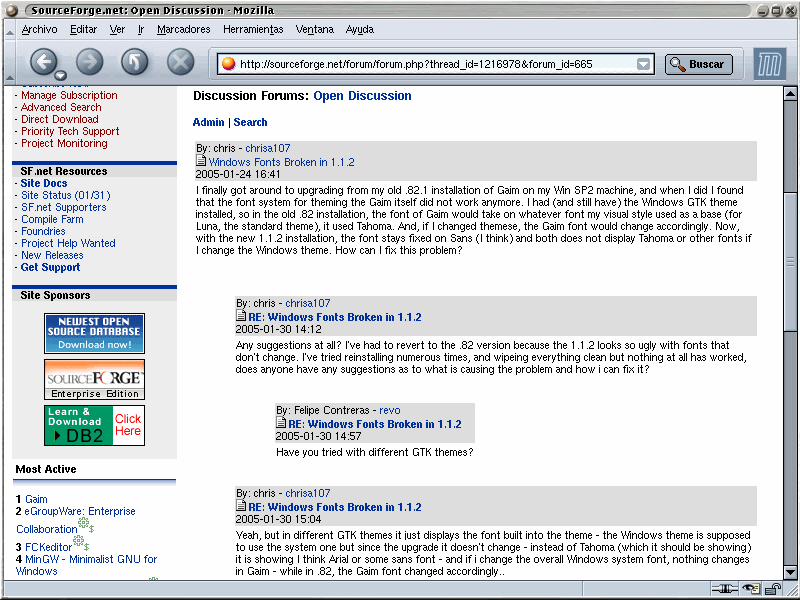
\includegraphics[bb=0 0 800 600, width=12cm, keepaspectratio]{img/foro1}
    \caption{Página con enlaces a hilos}
    \label{figura:foro_hilos}
 \end{figure}

A continuación un bloque ``verbatim'', que se utiliza para mostrar texto tal cual.
Se puede utilizar para ofrecer el contenido de correos electrónicos, código, entre otras cosas.

{\footnotesize
\begin{verbatim}
    From gaurav at gold-solutions.co.uk  Fri Jan 14 14:51:11 2005
    From: gaurav at gold-solutions.co.uk (gaurav_gold)
    Date: Fri Jan 14 19:25:51 2005
    Subject: [Mailman-Users] mailman issues
    Message-ID: <003c01c4fa40$1d99b4c0$94592252@gaurav7klgnyif>
    Dear Sir/Madam,
    How can people reply to the mailing list?  How do i turn off
    this feature? How can i also enable a feature where if someone
    replies the newsletter the email gets deleted?
    Thanks
    From msapiro at value.net  Fri Jan 14 19:48:51 2005
    From: msapiro at value.net (Mark Sapiro)
    Date: Fri Jan 14 19:49:04 2005
    Subject: [Mailman-Users] mailman issues
    In-Reply-To: <003c01c4fa40$1d99b4c0$94592252@gaurav7klgnyif>
    Message-ID: <PC173020050114104851057801b04d55@msapiro>
    gaurav_gold wrote:
    >How can people reply to the mailing list?  How do i turn off
    this feature? How can i also enable a feature where if someone
    replies the newsletter the email gets deleted?
    See the FAQ
    >Mailman FAQ: http://www.python.org/cgi-bin/faqw-mm.py
    article 3.11
\end{verbatim}
}

%%-- Objetivos del  proyecto
%%-- Si la sección anterior ha quedado muy extensa, se puede considerar convertir
%%-- Las siguientes tres secciones en un capítulo independiente de la memoria

\section{Objetivos del proyecto}
\label{sec:objetivos}

\subsection{Objetivo general} % título de subsección (se muestra)
\label{sec:objetivo-general} % identificador de subsección (no se muestra, es para poder referenciarla)


El objetivo de este Trabajo de Fin de Grado es comprobar la capacidad y eficiencia de una Raspberry Pi 4B para entrenar modelos de aprendizaje automático.\\

Aquí vendría el objetivo general en una frase:
Mi Trabajo Fin de Grado/Master consiste en crear de una herramienta de análisis de los comentarios jocosos en repositorios de software libre alojados en la plataforma GitHub.

Recuerda que los objetivos siempre vienen en infinitivo.


\subsection{Objetivos específicos}
\label{sec:objetivos-especificos}

Los objetivos específicos se pueden entender como las tareas en las que se ha desglosado el objetivo general. Y, sí, también vienen en infinitivo.

Lo mejor suele ser utilizar una lista no numerada, como sigue:

    \begin{itemize}
        \item Un objetivo específico.
        \item Otro objetivo específico.
        \item Tercer objetivo específico.
        \item \ldots
    \end{itemize}

\section{Planificación temporal}
\label{sec:planificacion-temporal}

Es conveniente que incluyas una descripción de lo que te ha llevado realizar el trabajo.
Hay gente que añade un diagrama de GANTT.
Lo importante es que quede claro cuánto tiempo has consumido en realizar el TFG/TFM 
(tiempo natural, p.ej., 6 meses) y a qué nivel de esfuerzo (p.ej., principalmente los 
fines de semana).

\section{Estructura de la memoria}
\label{sec:estructura}

Por último, en esta sección se introduce a alto nivel la organización del resto del documento
y qué contenidos se van a encontrar en cada capítulo.

    \begin{itemize}
      \item En el primer capítulo se hace una breve introducción al proyecto, se describen los objetivos del mismo y se refleja la planificación temporal.
      \item En el siguiente capítulo se describen las tecnologías utilizadas en el desarrollo de este TFM/TFG (Capítulo~\ref{chap:tecnologias}).
      \item En el capítulo~\ref{chap:diseño} Se describe el proceso de desarrollo
      de la herramienta \ldots
      \item En el capítulo~\ref{chap:experimentos} Se presentan las principales pruebas realizadas
      para validación de la plataforma/herramienta\ldots (o resultados de los experimentos
      efectuados).
      \item Por último, se presentan las conclusiones del proyecto así como los trabajos futuros que podrían derivarse de éste (Capítulo~\ref{chap:conclusiones}).
    \end{itemize}

\cleardoublepage

%%%%%%%%%%%%%%%%%%%%%%%%%%%%%%%%%%%%%%%%%%%%%%%%%%%%%%%%%%%%%%%%%%%%%%%%%%%%%%%%
%%%%%%%%%%%%%%%%%%%%%%%%%%%%%%%%%%%%%%%%%%%%%%%%%%%%%%%%%%%%%%%%%%%%%%%%%%%%%%%%
% ESTADO DEL ARTE %
%%%%%%%%%%%%%%%%%%%%%%%%%%%%%%%%%%%%%%%%%%%%%%%%%%%%%%%%%%%%%%%%%%%%%%%%%%%%%%%%

\chapter{Estado del arte}               %% a.k.a "Tecnologías utilizadas"
\label{chap:tecnologias}

Descripción de las tecnologías que utilizas en tu trabajo. 
Con dos o tres párrafos por cada tecnología, vale. 
Se supone que aquí viene todo lo que no has hecho tú.

Puedes citar libros, como el de Bonabeau et al., sobre procesos estigmérgicos~\cite{bonabeau:_swarm}. 
Me encantan los procesos estigmérgicos.
Deberías leer más sobre ellos.
Pero quizás no ahora, que tenemos que terminar la memoria para sacarnos por fin el título.
Nota que el \~ \ añade un espacio en blanco, pero no deja que exista un salto de línea. 
Imprescindible ponerlo para las citas.

Citar es importantísimo en textos científico-técnicos. 
Porque no partimos de cero.
Es más, partir de cero es de tontos; lo suyo es aprovecharse de lo ya existente para construir encima y hacer cosas más sofisticadas.
¿Dónde puedo encontrar textos científicos que referenciar?
Un buen sitio es Google Scholar\footnote{\url{http://scholar.google.com}}.
Por ejemplo, si buscas por ``stigmergy libre software'' para encontrar trabajo sobre software libre y el concepto de \emph{estigmergia} (¿te he comentado que me gusta el concepto de estigmergia ya?), encontrarás un artículo que escribí hace tiempo cuyo título es ``Self-organized development in libre software: a model based on the stigmergy concept''.
Si pulsas sobre las comillas dobles (entre la estrella y el ``citado por ...'', justo debajo del extracto del resumen del artículo, te saldrá una ventana emergente con cómo citar.
Abajo a la derecha, aparece un enlace BibTeX.
Púlsalo y encontrarás la referencia en formato BibTeX, tal que así:

\clearpage
{\footnotesize
\begin{minted}{bibtex}
@inproceedings{robles2005self,
  title={Self-organized development in libre software:
         a model based on the stigmergy concept},
  author={Robles, Gregorio and Merelo, Juan Juli\'an 
          and Gonz\'alez-Barahona, Jes\'us M.},
  booktitle={ProSim'05},
  year={2005}
}
\end{minted}
}

Copia el texto en BibTeX y pégalo en el fichero \texttt{memoria.bib}, que es donde están las referencias bibliográficas.
Para incluir la referencia en el texto de la memoria, deberás citarlo, como hemos hecho antes con~\cite{bonabeau:_swarm}, lo que pasa es que en vez de el identificador de la cita anterior (bonabeau:\_swarm), tendrás que poner el nuevo (robles2005self).
Compila el fichero \texttt{memoria.tex} (\texttt{pdflatex memoria.tex}), añade la bibliografía (\texttt{bibtex memoria.aux}) y vuelve a compilar \texttt{memoria.tex} (\texttt{pdflatex memoria.tex})\ldots y \emph{voilà} ¡tenemos una nueva cita~\cite{robles2005self}!

También existe la posibilidad de poner notas al pie de página, por ejemplo, una para indicarte que visite la página del GSyC\footnote{\url{http://gsyc.es}}.

En este apartado se reaizará una breve descripción del dispositivo principal, que es motivo de esta investigación. También se expondrá todo el software que se ha necesitado instalar para poder implementar los modelos y ponerlos a prueba.

\section{Machine Learning e IoT}
\label{sec:machine_learning}

El objetivo princicpal de este trabajo de investigación es conocer si la Raspberry es un dispositivo lo suficientemente potente para realizar tareas de Machine learning es por ello que primero debemos tener claros estos conceptos para poder entender el proyecto.

 Machine Learning o aprendizaje automático, es una disciplina del campo de la Inteligencia Artificial que permite a las máquinas aprender sin ser explícitamente programadas para ello. Para aprender utilizan algoritmos que permiten a los ordenadores identificar los patrones que existen en grandes cantidades de datos y utilizar estos patrones para poder elaborar predicciones del futuro. 
 
 Los datos que se proporcionan al algoritmo normalmente son ficheros con varias filas y columnas. Cada fila representa un ejemplo de datos que se pasa al modelo para entrenar. Mientras que si posee varías columnas significa que hay varios valores que definen un ejemplo, se dice que estas columnas son las caracterísitcas del dataSet. 
 
 Un ejemplo de lo que contiene un dataSet es la tabla~\ref{tab:my_dataSet}, donde se proporciona información sobre cuando un niño va a jugar a la pelota o no. En este caso tendríamos tres características (previsión, temperatura y amigos), la columna jugar es la decisión que tome el niño ante los valores de esas caracterísitcas. Por lo tnato, cada fila define una situación diferente, es decir es un ejemplo de lo que puede suceder.
 
 \begin{table}[]
     \centering
     \begin{tabular}{| c | c | c | c |}
            \hline
          Previsión & Temperatura & Amigos & Jugar\\
          \hline
           Soleado &  25 ºC & 2 & Si \\
           \hline
           Lluvioso &  12 ºC & 0 & No\\
           \hline
           Nublado &  18 ºC & 4 & Si\\
           \hline
     \end{tabular}
     \caption{Ejemplo de un dataSet}
     \label{tab:my_dataSet}
 \end{table}
 
 Los algoritmos de Machine Learning se dividen en tres categorías: 

\begin{itemize}
    \item \textbf{Aprendizaje supervisado}. En este tipo de aprendizaje se le proporciona al algoritmo un conjunto de datos de entrada con su salida correspondiente. De esta forma el programa puede "aprender" la relación que existe entre la salida y el conjunto de entradas. Dependiendo del tipo de salida podremos encontrar dos clases de modelos: modelos de regresión o de clasificación.
    
    Si la salida es un valor numérico continuo, estaríamos ante un problema de regresión en el que se busca obtener la recta que mejor se ajusta a los datos de entrada para poder predecir otros valores. Si, en cambio, la salida es una etiqueta de clase, es decir un valor discreto, se correspondería a un problema de clasificación, en los que se busca estimar a qué clase pertenecen los datos de entrada. 
    
    Un ejemplo de este último tipo se puede ver en la Figura~\ref{fig:a_supervisado}, donde cada una de las formas serían las entradas y las etiquetas de: triángulo, cuadrado o círculo serían la salidas, cada dato de entrada tiene asignada una de estas etiquetas. Todo esto formaría lo que se denomina dataSet que es el conjunto de datos que se pasan al modelo para entrenar y poder encontrar esas relaciones entre entradas y salidas. En este caso cuando al modelo se le pregunte a qué clase pertenece una figura (del mismo tipo que ha visto durante el entrenamiento), si es lo suficientemente robusto, debería de ser capaz de identificarlo como un cuadrado.
    
    \begin{figure}[h!]
      \centering
      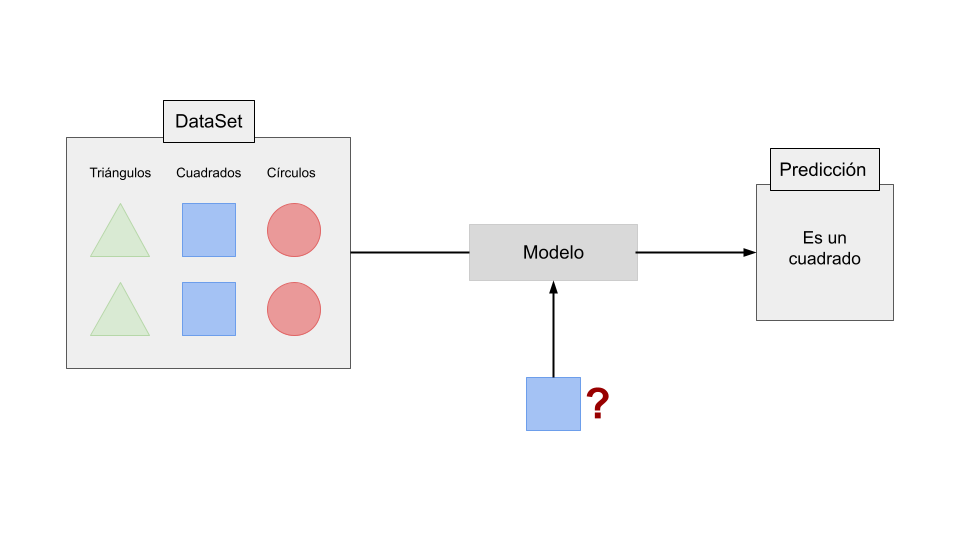
\includegraphics[width=12cm, keepaspectratio]{img/a_supervisado.png}
      \caption{Estructura aprendizaje supervisado para clasificación.}\label{fig:a_supervisado}
    \end{figure}
    
    Existen multitud de modelos de Machine Learning que sirven para resolver problemas mediante aprendizaje supervisado, como por ejemplo algoritmos de Regresión logística, Árboles de decisión, Máquinas de soporte vectorial...
    
    \item \textbf{Aprendizaje no supervisado}. Al algoritmo de aprendizaje se le proporciona únicamente el conjunto de datos de entrada, sin ningún tipo de dato de salida. El objetivo es que el método de aprendizaje utilizado detecte posibles patrones de interés en el conjunto de datos de entrada. 
    
    \begin{figure}[h!]
      \centering
      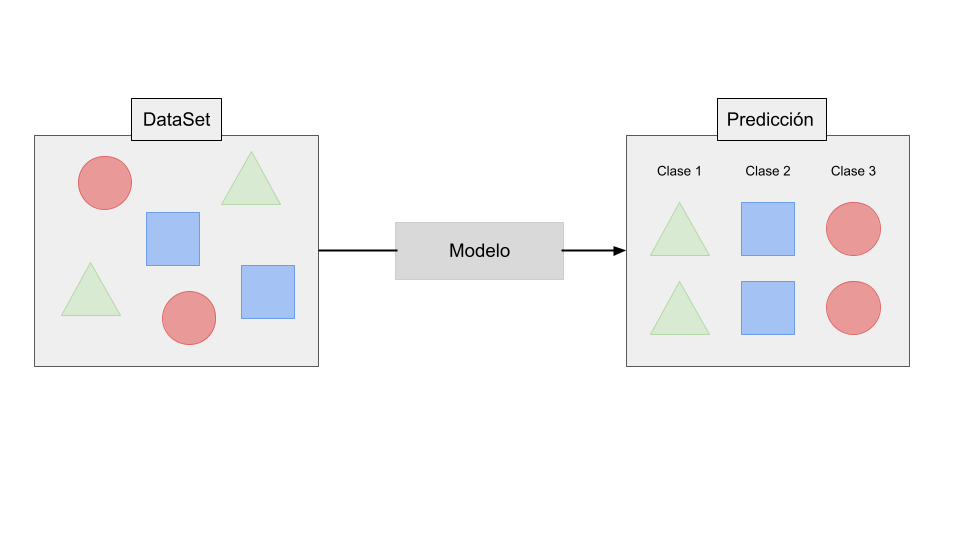
\includegraphics[width=12cm, keepaspectratio]{img/a_no_supervisado.png}
      \caption{Estructura aprendizaje no supervisado para segmentación.}\label{fig:a_no_supervisado}
    \end{figure}
    
    Hay principalmente dos tipos de tareas que estos algoritmos tratan de realizar. Una de ellas es el clustering (o segmentación), que sirve para encontrar diferentes grupos dentro de los datos de entrada. En la Figura~\ref{fig:a_no_supervisado} se muestra un ejemplo esquemático de la ejecución de un problema de este estilo, donde una vez más las entradas serían cada una de las formas pero en esta ocasión no están etiquetadas como veíamos en la Figura~\ref{fig:a_supervisado}. El modelo en esta ocasión, viendo las características de cada uno de los datos, los agrupará en diferentes clases.
    
    La otra misión que pueden tener este tipo de aprendizaje es reducir la dimensionalidad de los datos, es decir, reducir el número de características del conjunto de datos de entrada asumiendo que muchas de ellas son redundantes y por lo tanto no aportan información nueva.
    
    Al igual que en aprendizaje supervisado existen varios algoritmos que buscan resolver estas tareas, como por ejemplo el método KNN, K-Means...
    
    \item \textbf{Aprendizaje por refuerzo}. El algoritmo aprende a desarrollar la tarea que se le asigna a base de un esquema de recompensas y penalizaciones ante las decisiones que toma el programa en cada una de las iteraciones.
\end{itemize}

Gracias a que estos algoritmos pueden estar aprendiendo constantemente de nuevos datos consiguen ir perfeccionando su comportamiento, lo que hace que las técnicas de Machine Learning sean cada vez más importantes debido a la multitud de aplicaciones que se le pueden dentro de la robótica, los vehículos autónomos, diagnósticos médicos, markenting....

Uno de los campos en los que son de gran importancia estas técnicas es en los proyectos de IoT (Internet of Things). El Internet de las cosas (o Internet of Things) es la interconexión de sensores y dispositivos, como por ejemplo pueden ser los electrodomésticos, termostátos, coches, ropa... Todos ellos se conectan a través de una red por medio de la cual pueden interaccionar y compartir datos. En estos casos se utiliza Machine Learning para generar, por medio de todos estos datos recopilados, nuevos modelos de aprendizaje automático cuyas predicciones se pueden usar para poder actuar sobre el entorno. Las posibles aplicaciones que ofrece esto son prácticamente infinitas, algunos ejemplos pueden ser:

\begin{itemize}
    \item Riego de plantas. Tomando medidas de luz, humedad, temperatura...Por medio de ML se puede automatizar el riego de las plantas.
    \item Sistema antirobo. 
    \item Telemedicina. Por medio de dispositivos que lleve puesto el paciente se puede tener un control sobre su estado de salud e incluso hacer diagnósticos anticipados.
    \item Control de luces. Apagar o encender de forma totalmente autónoma las luces si hay o no una persona en la habitación.
\end{itemize}

\section{Dispositivo Hardware: Raspberry Pi 4 Modelo B}
\label{sec:dispositivo_hardware}

Raspberry Pi\footnote{\url{https://www.raspberrypi.org/}} es un ordenador de bajo coste y tamaño reducido desarrollado por Raspberry Pi Foundation. Este dispositivo se puede emplear en  multitud de aplicaciones pero su principal objetivo es hacer accesible la informática a todos los usuarios. A parte de poder realizar todas las tareas que se esperan de un ordenador, también puede interactuar con el entorno a través de sensores conectados a sus pines GPIO.

El sistema operativo que ofrece es Raspbian Pi OS, una versión adaptada de Debian. Sin embargo permite utilizar otros sistemas.

Desde su primer lanzamiento se han ido desarrollando y comercializado nuevos modelos. En este proyecto se utilizará la última versión de estos dispositivos denominado como Raspberry Pi 4 Modelo B con 4GB de RAM. Dicho modelo posee un total de 40 pines GPIO, 2 puertos micro HDMI y 4 puertos USB. Puede realizar conexiones inalámbricas ya que tiene Bluetooth 5.0 y Wi-Fi, aun que también puede utilizar Ethernet. Por último la alimentación viene dada por un cable USB de tipo C con el que puede alcanzar un total de 1.2 A.

Dicho modelo posee un procesador ARM Cortex-172 con un total de cuatro cores físicos y cuatro lógicos. Otro detalle destacable de la Raspberry para el desarrollo de este trabajo es que posee una arquitectura SMP (Symmetric Multi-Processing), un tipo de arquitectura de computador en el que las unidades de procesamiento comparten una única memoria central, lo que permite que cualquier procesador trabaje en cualquier tarea sin importar su localización en memoria. 

Actualmente es uno de los dispositivos más populares ya que brinda un sinfín de posibilidades a pesar de su pequeño tamaño. Específicamente dentro de el campo de aprendizaje automático e IoT se podrían desarrollar multitud de aplicaciones gracias a la interacción que tiene con el entorno por medio de los sensores y actuadores que se pueden conectar. Por ello, en este trabajo de investigación se busca examinar el rendimiento de este pequeño ordenador y comprobar hasta donde se podría llegar con él, dentro del campo del aprendizaje automático. 


\begin{comment}

\begin{table}
 \begin{center}
  \begin{tabular}{ | l | c | r |} % tenemos tres colummnas, la primera alineada a la izquierda (l), la segunda al centro (c) y la tercera a la derecha (r). El | indica que entre las columnas habrá una línea separadora.
    \hline
    Uno & 2 & 3 \\ \hline % el hline nos da una línea vertical
    Cuatro & 5 & 6 \\ \hline
    Siete & 8 & 9 \\
    \hline
  \end{tabular}
  \caption{Ejemplo de tabla. Aquí viene una pequeña descripción (el \emph{caption}) del contenido de la tabla. Si la tabla no es autoexplicativa, siempre viene bien aclararla aquí.}
  \label{tabla:ejemplo}
 \end{center}
\end{table}
\end{comment}

\section{Sistema Operativo: Ubuntu 21.10} 
\label{sec:sistema_operativo}

El sistema operativo Ubuntu\footnote{\url{https://ubuntu.com/}} es una distribución de código abierto basada en Debian, está compuesto de software normalmente distribuido bajo una licencia libre o de código abierto. La empresa responsable de su creación y mantenimiento es Canonical, una empresa de programación de ordenadores con base en Reino Unido fundada por el empresario Mark Shuttleworth.

La primera versión de Ubuntu fue la 4.10 lanzada el 20 de Octubre de 2004. A partir de la versión 13.4 las versiones estables sin soporte a largo plazo se liberan cada seis meses, y Canonical proporciona soporte técnico y actualizaciones de seguridad durante 9 meses. Las versiones LTS (Long Term Support) ofrecen un soporte técnico durante 5 años a partir de la fecha de lanzamiento.

La última versión fue lanzada el 14 de Octubre de 2021, que es la versión Ubuntu 21.10. Dicha versión utiliza el kernel 5.13, con cambios y mejoras para componentes que daban problemas. También tiene un nuevo instalador, escrito desde cero en Flutter, que facilita la instalación del sistema operativo. Una de las novedades más importantes es que actualiza su escritorio a GNOME 40. 


\subsection{Gestor de paquetes: Miniforge}
\label{subsec:gestor_de_paquetes}

%%-- El comando \gls{} permite incluir términos en el glosario, para luego reunirlos todos
%%-- en una tabla al comienzo o al final del documento, junto con sus definiciones.

Miniforge es un instalador mínimo de conda especifico de conda-forge, que permite instalar el manejador de paquetes conda con una serie de configuraciones predifinidas. Es muy similar a un instalador de Miniconda.

Miniconda es un sistema de gestión de paquetes y entornos virtuales. Mediante él se instala una pequeña versión de arranque de Anaconda que incluye solo conda, Python, los paquetes de los que dependen y otros pocos paquetes útiles como pueden ser pip, zlib...

Ofrece casi lo mismo que Anaconda pero es mucho más ligero, lo que lo hace idóneo para poder desarrollar el proyecto en el dispositivo utilizado. Además, facilita la replicación de un entorno concreto ya que permite tener un mayor control y orden sobre los paquetes que se instalan. 

\section{Lenguaje de programación: Python}
\label{sec:lenguaje_de_programación}

Python\footnote{\url{https://www.python.org/}} es un lenguaje de programación que nace a principios de los años 90 gracias al informático holandés Guido Van Rossum. Su objetivo era crear un lenguaje de programación que fuera fácil de aprender, escribir y entender.

Es un lenguaje de alto nivel (sencillo de leer y escribir debido a su similitud con el lenguaje humano), interactivo, interpretado y orientado a objetos. Al ser interpretado permite poder ejecutarlo sin necesidad de compilarlo previamente, reduciendo el tiempo entre la escritura y la ejecución del código. Utiliza módulos y paquetes, lo que fomenta la modularidad y la reutilización de código. 

Además es multiplataforma y de código abierto, por lo tanto gratuito, lo que ha ayudado a que Python sea el lenguaje con mayor crecimiento y uno de los más utilizados en la actualidad.  

Entre los campos en los que más se emplea este lenguaje se encuentra la inteligencia artificial, big data, machine learning y data science entre otros, ya que facilita la creación de códigos entendibles de rápido aprendizaje como los que son necesarios en este tipo de proyectos.

\subsection{Entorno de desarrollo: Jupyter-notebook}
\label{subsec:entorno_de_desarrollo}

Jupyter-notebook es una aplicación web lanzada en 2015, de código abierto desarrollada por la organización Proyecto Jupyter. Permite crear y compartir documentos computacionales que siguen un esquema versionado y una lista ordenada de celdas de entrada y salida.

Estas celdas pueden contener código, texto en formato Markdown, fórmulas matemáticas y ecuaciones, o también contenido multimedia. Cada celda se puede ejecutar para visualizar los datos y ver los resultados de salida. Los documentos creados en Jupyter pueden exportarse en otros formatos como PDF, Python o HTML. Además se puede utilizar tanto remotamente como en local.

Los dos componentes principales de Jupyter Notebook son un conjunto de núcleos (intérpretes) y el Dashboard. Es compatible con 49 núcleos que permiten trabajar en diferentes lenguajes como R, Julia, C++ o Java. Sin embargo, el kernel que utiliza por defecto es IPython para programar con Python. 

\subsection{Librerías}
\label{subsec:Librerías}
Para el desarrollo del proyecto se utilizaron varias librerías que permitiesen la creación de códigos de aprendizaje automático. A continuación se hace mención de las principales y más importantes.

\subsubsection{Scikit-learn}
\label{subsubsec:Scikit-learn}
Scikit-Learn\footnote{\url{https://scikit-learn.org/stable/}} es una librería, escrita principalmente en Python, que cuenta con algoritmos de clasificación, regresión, clustering y reducción de dimensionalidad. Fue inicialmente desarrollada por David Cournapeau como proyecto de Google Summer of code en 2007.

La gran variedad de algoritmos y utilidades de Scikit-learn la convierten en una herramienta muy eficaz para generar aplicaciones de aprendizaje automático.

\subsubsection{Pandas}
\label{subsubsec:Pandas}

Pandas\footnote{\url{https://pandas.pydata.org/}} es una librería de Python de código abierto especializada en el manejo y análisis de estructuras de datos. Es muy útil en el ámbito de Data Science y Machine Learning, ya que ofrece unas estructuras muy poderosas y flexibles que facilitan la manipulación y tratamiento de datos.

Tiene todas las funcionalidades necesarias para el análisis de datos como pueden ser: cargar, modelar, analizar, manipular y preparar los datos.

\begin{comment}
PyCharm es un \gls{ide} dedicado concretamente a la programación en Python y desarrollado por la compañía checa JetBrains.

Proporciona análisis de código, un depurador gráfico, una consola de Python integrada, control de versiones y, además, soporta desarrollo web con Django. Todas estas características lo convierten en un entorno completo e intuitivo, idóneo para el desarrollo de proyectos académicos como el que nos ocupa.
\end{comment}

\section{Sensores}
\label{sec:sensores}

En este proyecto también se utilizaron sensores para tomar medidas del entorno y generar nustro propio dataSet con el que entrenar los modelos de aprendizaje automático. En concreto se utilizaron dos: una fotoresistencia (LDR) y un sensor BME280, a continuación se darán más detalles de ambos sensores.

\subsection{Fotoresistencia}
\label{subsec:fotoresistencia}

Esta resistencia también denominada como LDR por sus siglas en inglés Light Dependent Resistor, varía su resistencia dependiendo de la cantidad de luz que incida sobre su superficie. Funciona gracias al principio de la fotoconductividad que es un fenómeno óptico en el que la conductividad del material aumenta cuando la luz es absorvida. Luego cuando la luz cae sobre la resistencia los electrones son excitados lo que provoca que empiece a fluir cada vez más corriente a través del dispositivo, por lo tanto la resistencia del dispositivo dismimnuye. Por lo tanto cuando la LDR recibe luz, su resistencia será más baja y cuando esté a oscuras la resistencia será más alta. La resistencia del LDR está en torno a los $5 k\Omega$

Para que la Raspberry pueda obtener el valor que sensa este dispositivo es necesario utilizar un conversor. En este caso utilizaremos el HW-103 con el que al conectarlo a la Raspberry y a el sensor podremos conseguir una señal digital. Cuando a la Raspberry le llegue un cero significará que hay luz mientras que si lee un uno es que no hay luz.

\subsection{BME280}
\label{subsec:bme280}

El sensor BME280\footnote{\url{https://www.bosch-sensortec.com/products/environmental-sensors/humidity-sensors-bme280/}}, desarrollado por Bosh, es un sensor desarrollado especialmente para aplicaciones móviles y prendas de vestir donde el tamaño y el bajo consumo de energía son elementos claves. Integra en un mismo dispositivo tres sensores diferentes que proveen medidas de alta precisión. Los tres sensores que posee son: uno de temperatura, otro de presión atmosférica y por último, humedad relativa. 

El rango de la temperatura va desde los $-40\, \mbox{ºC}$ hasta los $85\, \mbox{ºC}$, con una precisión de $\pm 0.5\, \mbox{ºC}$. El sensor de presión tiene un rango de entre $300 hPa$ y $1100 hPa$. Por útlimo el rango de la humedad relativa va desde el 0 hasta el 100\%.

La comunicación con este sensor es muy sencilla ya que puede usar tanto I2C o SPI. Tiene una tensión de funcionamiento de $3.3V$. Y a pesar de que integra tres sensores diferentes su tamaño es pequeño, de $19x18 mm$.

Este tipo de sensores se utilizan en aplicaciones como: monitorización del clima, automatización del hogar, sistemas de autopiloto para drones...

\section{Redacción de la memoria: LaTeX/Overleaf}
\label{sec:redaccion_de_la_memoria}

LaTeX es un sistema de composición tipográfica de alta calidad que incluye características especialmente diseñadas para la producción de documentación técnica y científica. Estas características, entre las que se encuentran la posibilidad de incluir expresiones matemáticas, fragmentos de código, tablas y referencias, junto con el hecho de que se distribuya como software libre, han hecho que LaTeX se convierta en el estándar de facto para la redacción y publicación de artículos académicos, tesis y todo tipo de documentos científico-técnicos. 

Por su parte, Overleaf es un editor LaTeX colaborativo basado en la nube. Lanzado originalmente en 2012, fue creado por dos matemáticos que se inspiraron en su propia experiencia en el ámbito académico para crear una solución satisfactoria para la escritura científica colaborativa.

Además de por su perfil colaborativo, Overleaf destaca porque, pese a que en LaTeX el escritor utiliza texto plano en lugar de texto formateado (como ocurre en otros procesadores de texto como Microsoft Word, LibreOffice Writer y Apple Pages), éste puede visualizar en todo momento y paralelamente el texto formateado que resulta de la escritura del código fuente.

\cleardoublepage

%%%%%%%%%%%%%%%%%%%%%%%%%%%%%%%%%%%%%%%%%%%%%%%%%%%%%%%%%%%%%%%%%%%%%%%%%%%%%%%%
%%%%%%%%%%%%%%%%%%%%%%%%%%%%%%%%%%%%%%%%%%%%%%%%%%%%%%%%%%%%%%%%%%%%%%%%%%%%%%%%
% DISEÑO E IMPLEMENTACIÓN %
%%%%%%%%%%%%%%%%%%%%%%%%%%%%%%%%%%%%%%%%%%%%%%%%%%%%%%%%%%%%%%%%%%%%%%%%%%%%%%%%

\chapter{Diseño e implementación}
\label{chap:diseño}


\begin{comment}
Aquí viene todo lo que has hecho tú (tecnológicamente). 
Puedes entrar hasta el detalle. 
Es la parte más importante de la memoria, porque describe lo que has hecho tú.
Eso sí, normalmente aconsejo no poner código, sino diagramas.
\end{comment}

En este capítulo se realiza una descipción detallada sobre la arquitecura del proyecto, las instalaciones necesarias para poder realizar el trabajo, una breve explicación sobre los modelos de aprendizaje que se implementaron así como los data sets utilizados.

\section{Arquitectura general} 
\label{sec:arquitectura}

Ante la gran importancia que están adquiriendo las aplicaciones de Machine Learning e IoT en las últimas decadas, este proyecto busca examinar la capacidad de la Raspberry para utilizarla como un dispositivo en el que se puedan implementar y desarrollar este tipo de tareas. El pequeño tamaño, su bajo coste y su capacidad de interacción con el entorno hacen que la Raspberry sea una buena opción para algoritmos con estos fines. 

Sin embargo, no nos podemos fiar únicamente de las apariencias. Hay que averiguar si verdaderamente un dispositivo como este, con menos recursos que un ordenador común, puede llevar a cabo tareas de este estilo con éxito.

Para ello, y como se explicará en mayor detalle en los siguientes capítulos, pondremos a prueba a la máquina con diferentes pruebas. En la Figura~\ref{fig:arquitectura} se puede visualizar un esquema general de en qué consisten dichas pruebas. Como se puede ver en esta figura los experimentos se llevarán a cabo tanto en la Raspberry como en un portátil para poder comparar los resultados y comprender mejor los resultados obtenidos en la Raspberry.


\begin{figure}[h!]
  \centering
  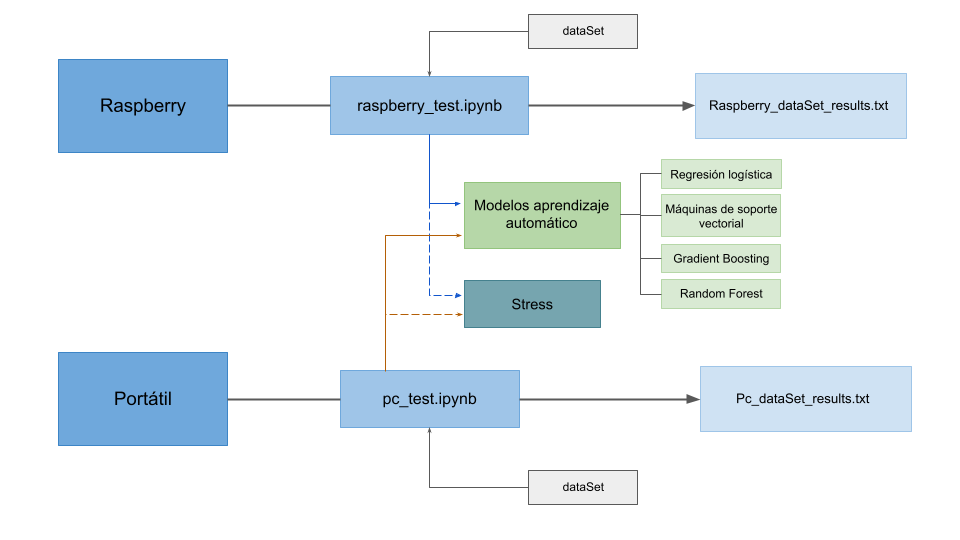
\includegraphics[width=14cm, keepaspectratio]{img/arquitectura_general.png}
  \caption{Estructura de los experimentos}\label{fig:arquitectura}
\end{figure}

Como se explicó en la sección~\ref{sec:machine_learning} hay varios tipos de aprendizaje automático y dentro de cada clase existen aún más métodos para resolver un mismo problema de formas diferentes. En este proyecto utilizaremos algoritmos de aprendizaje supervisado para realizar problemas de clasificación binaria, es decir, solo existen dos clases a las que pueden pertenecer los datos. Concretamente (y como se puede ver en la Figura~\ref{fig:arquitectura}) se utilizarán cuatro algoritmos de Machine Learning que son: Regresión logística, Máquinas de soporte vectorial, Gradient boosting y Random forest.

Aprovechando los puertos GPIO de los que está provista la Raspberry se utilizaron un par de sensores para poder generar un nuevo dataSet que utilizar para entrenar los modelos de aprendizaje automático.

En la Figura~\ref{fig:esquema_sensores} se puede observar la estructura de como se lleva a cabo la recolección de información de los sensores por parte de la Raspeberry. Con todo conectado correctamente, se generará un nuevo fichero csv con los datos medidos durante el tiempo que el usuario haya estado ejecutando dicho programa. Dicho dataSet podrá utilizarse para entrenar los modelos de aprendizaje. Además mediante al información recogida se creará una figura que contiene los datos sensados en cada instante de tiempo.

\begin{figure}[h!]
  \centering
  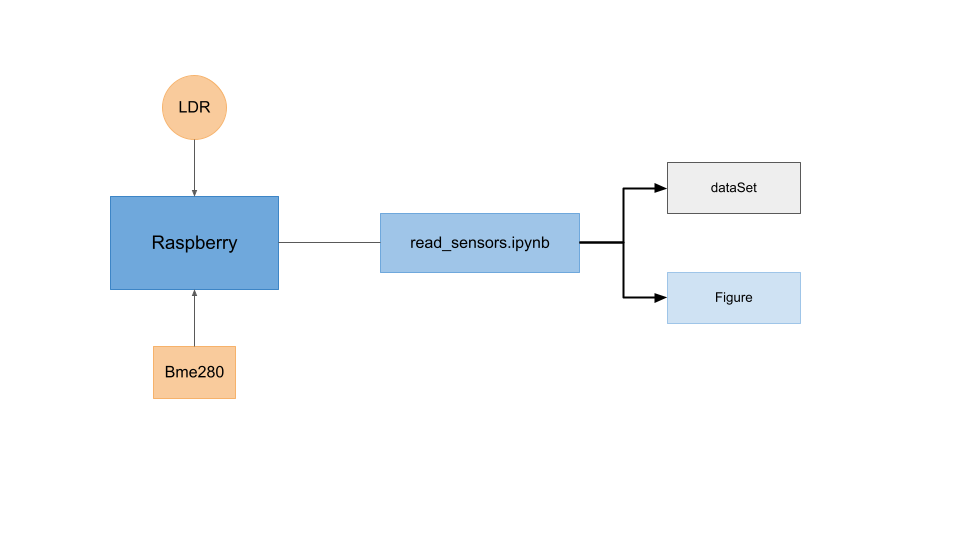
\includegraphics[width=14cm, keepaspectratio]{img/esquema_sensores.png}
  \caption{Estructura generación de un nuevo de dataSet}\label{fig:esquema_sensores}
\end{figure}

Antes de adentrarnos en una explicación en mayor profundadidad de lo que se desarrolla en este proyecto

Si tu proyecto es un software, siempre es bueno poner la arquitectura (que es cómo se estructura tu programa a ``vista de pájaro'').

Por ejemplo, puedes verlo en la Figura~\ref{fig:arquitectura}.
\LaTeX \ pone las figuras donde mejor cuadran. 
Y eso quiere decir que quizás no lo haga donde lo hemos puesto\ldots
Eso no es malo.
A veces queda un poco raro, pero es la filosofía de \LaTeX: tú al contenido, que yo me encargo de la maquetación.

\begin{comment}[]
\begin{figure}
  \centering
  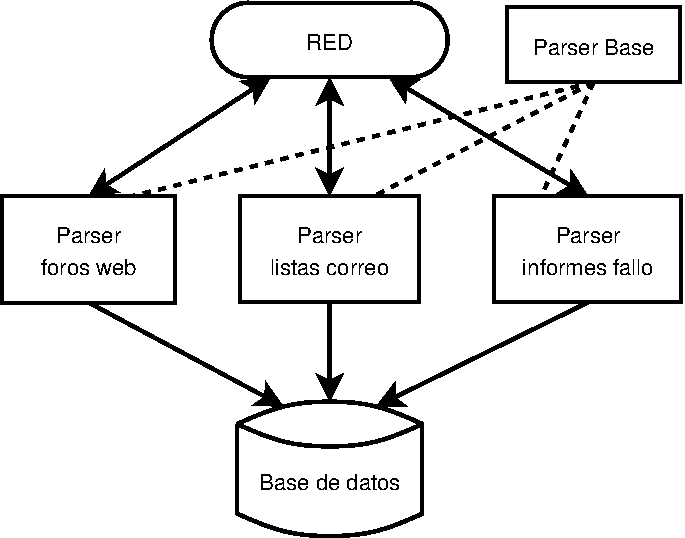
\includegraphics[width=9cm, keepaspectratio]{img/arquitectura.png}
  \caption{Estructura del parser básico.}\label{fig:arquitectura}
\end{figure}

\begin{figure}
    \centering
    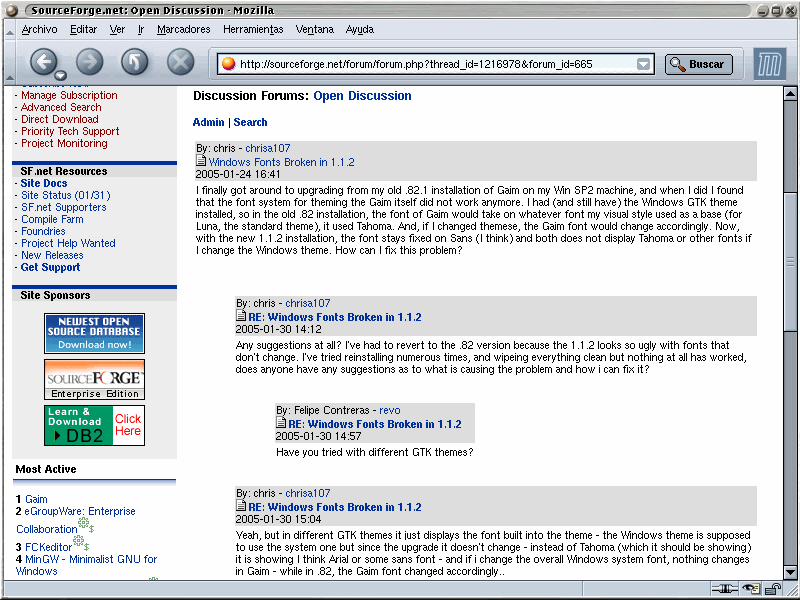
\includegraphics[bb=0 0 800 600, width=12cm, keepaspectratio]{img/foro1}
    \caption{Página con enlaces a hilos}\label{fig:_arquitectura}
\end{figure}
\end{comment}
 
Recuerda que toda figura que añadas a tu memoria debe ser explicada.
Sí, aunque te parezca evidente lo que se ve en la Figura~\ref{fig:arquitectura}, la figura en sí solamente es un apoyo a tu texto.
Así que explica lo que se ve en la Figura, haciendo referencia a la misma tal y como ves aquí.
Por ejemplo: En la Figura~\ref{fig:arquitectura} se puede ver que la estructura del \emph{parser} básico, que consta de seis componentes diferentes: los datos se obtienen de la red, y según el tipo de dato, se pasará a un \emph{parser} específico y bla, bla, bla\ldots

Si utilizas una base de datos, no te olvides de incluir también un diagrama de entidad-relación.


\section{Configuración del entorno}

Para poder desarrollar correctamente este trabajo es necesario preparar adecuadamente el entorno, una vez acondicionado todo se dará pie al motivo principal de esta investigación.

El primer paso para esto fue montar adecuadamente la Raspberry Pi conforme las instrucciones de Okdo\footnote{\url{https://www.okdo.com/getstarted/}}, empresa de la que procede el kit con el hardware utilizado en el proyecto.

Una vez está listo el hardware hay que instalar el software necesario para la generación de modelos de machine learning.
Comenzando por cambiar el sistema operativo, en vez de utilizar el que viene por defecto, Raspbian Pi OS, se instaló Ubuntu 21.10\footnote{\url{https://ubuntu.com/tutorials/how-to-install-ubuntu-desktop-on-raspberry-pi-4}}.

A continuación se instaló Miniforge, por medio del cual se crea un entorno virtual donde se instalaron todos los paquetes necesarios para el proyecto como son scikit-learn, pandas, jupyter-notebook... Estos paquetes permitirán desarrollar modelos de aprendizaje automático.

Además se instaló stress, un comando de Linux que sirve para estresar durante un tiempo que se le indique el número de cpus que se le especifican. En este caso, dicho comando se utilizará para poder someter a la Raspberry a diferentes niveles de carga computacional y de este modo ver su capacidad para entrenar modelos de aprendizaje automático. 

En el Anexo de esta memoria se podrá encontrar en mayor detalle las dificultades y las soluciones a los problemas hallados a la hora de realizar todo lo comentado en este apartado.


\subsection{Conexión de los sensores}
\label{subsec:conexion_sensores}

Como se comentaba en el capítulo~\ref{sec:sensores}, en este proyecto se utilizaron en total dos sensores, un LDR y un sensor BME280. Para obtener las medidas sensadas hubo que conectar ambos tal y como se puede ver en la Figura~\ref{fig:circuito}.

\begin{figure}[h!]
  \centering
  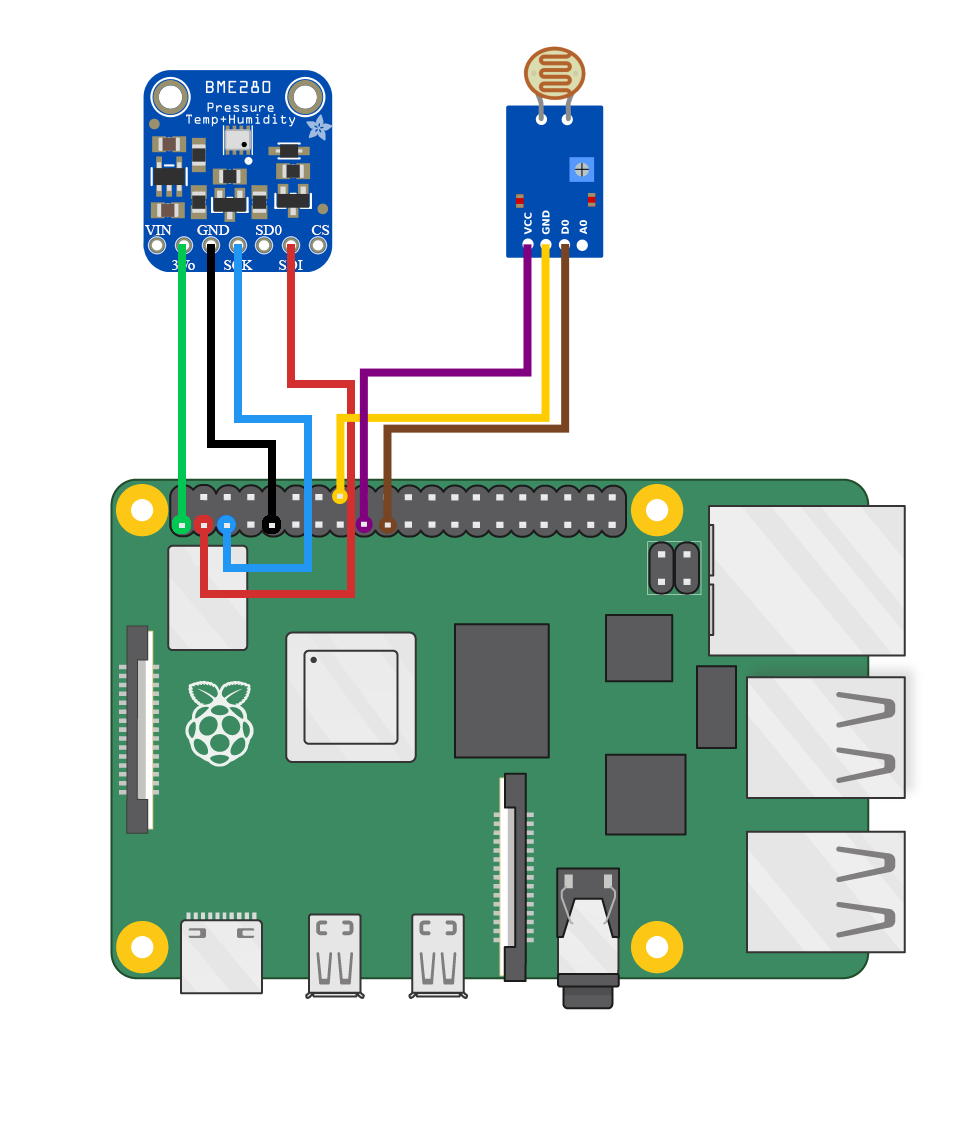
\includegraphics[width=9cm, keepaspectratio]{img/circuito.png}
  \caption{Conexiones de los sensores a la Raspberry.}\label{fig:circuito}
\end{figure}

En el caso del sensor BME280 se utiliza comunicación por I2C para poder leer las medidas de temperatura, humedad y presión, por eso está conectado a los pines dos y tres de la Raspberry. Mientras que el LDR se conecta al pin 10 para saber si hay luz o no.

Para poder obtener los valores del LDR fue necesario instalar el paquete LGPIO, los detalles de su instalación se encuentran en el Anexo.

Para la comunicación I2C hubo que instalar el paquete \textit{i2c-tools} en la Raspberry. Para poder utilizar este paquete es necesario tener permisos de root, sin embargo se dieron permisos a un usuario de forma que no tuviese que ser root para poder ejecutarlo\footnote{\url{https://lexruee.ch/setting-i2c-permissions-for-non-root-users.html}}. Dentro del entorno de conda donde se desarrolla el proyecto se tuvieron que instalar además otros dos paquetes: \textit{smbus2} y \textit{RPi.bme280}.

\section{Modelos de aprendizaje automático}

Con el entorno preparado se generaron mediante scripts de Python cuatro modelos diferentes de aprendizaje supervisado para realizar una clasificación binaria. Utilizando la librería scikit-learn se generaron un modelo de Regresión logística, otro de Máquinas de soporte vectorial, Gradient boosting y un último de Random forest.

\subsection{Regresión logística}
\label{subsec:regresion_logistica}

Modelo de aprendizaje supervisado que realiza tareas de clasificación binaria, es decir solo existen dos posibles clases. Esta técnica busca una función acotada (normalmente entre 0 y 1) que divida los datos de ambas clases de forma bien diferenciada. Normalmente dicha función se denomina como logística o sigmoide y se define de la siguiente forma:

\begin{equation}
    h_w(x^{(i)}) = \frac{1}{1 + e^{\sum_{j=0}^{d} w_j x_j^{(i)} }}
\end{equation}

Dicha expresión devolverá un valor entre cero y uno. Según lo próximo que este el valor a cero o uno pertenecerá a una clase u otra. 

Los parámetros representados por $w$ son los pesos que utiliza la función para realizar la predicción. Cada peso está multiplicando a una caracerística, simbolizada mediante $x_j$. Luego, para conocer a qué clase pertenece el ejemplo $x^{(i)}$ habrá que aplicar la fórmula anterior y por lo tanto se tendrá que realizar el sumatorio de todos los pesos multiplicados por sus respectivas caracterísitcas (desde la cero hasta la d-ésima). 

Durante la fase de entrenamiento el modelo ajusta los pesos mediante un método de optimización, a fin de que las predicciones que se realicen mediante ellos tengan el mínimo error posible. Para obtener los valores óptimos de los pesos se utiliza el método de descenso por gradiente, mediante el cual se irán actualizando los valores de los pesos conforme vaya entrenando con más ejemplos. La función de descenso por gradiente se define de la siguiente manera:

\begin{equation}
    w_j = w_j - \alpha \frac{1}{n} \sum_{i= 1}^{n} (h_w(x^{(i)}) - y^{(i)}) x_j^{(i)}
\end{equation}

Para calcular los pesos se utiliza el error que existe entre la salida predecida con los pesos estimados hasta ahora ($h_w(x^{(i)})$) y el valor real, es decir, la salida que verdaderamente corresponde a ese ejemplo ($y^{(i)}$). También es necesario definir el valor del ratio de aprendizaje ($\alpha$), si se le da un valor muy elevado puede llegar a no converger el modelo en ninguna solución. Esto se realiza para todos los valores de $j$, desde $j= 0$ hasta $j= d$, que es el número total de caracterísitcas.

Se dará por finalizada la fase de aprendizaje cuando se consiga que los valores de los pesos minimicen una función de coste:

\begin{equation}
    J(w) = \frac{1}{2} \sum_{i= 1}^{n} {(h_w(x^{(i)}) - y^{(i)})}^2 
\end{equation}

En scikit-learn por medio de la función LogisticRegression\cite{LogisticRegressionDoc}, que pertenece a la librería \textit{sklearn.linear\_model}, se puede generar este modelo de aprendizaje automático para entrenarlo y posteriormente predecir con él. 

Entre los parámetros que se pueden asignar a esta función hay dos que son destacables. El primero de ellos es \textit{max\_iter}, máximo número de iteraciones que se permiten para encontrar la solución que converja, por defecto tiene un valor igual a 100. Por otra párte está el parámetro \textit{n\_jobs}, que permite declarar el número de cpus que se desean utilizar para paralelizar el proceso. Sin embargo, la asignación de este valor solo tiene efecto si se realiza una clasificación multiclase, de lo contrario utilizará un único core independientemente del valor asignado.

\subsection{Máquinas de soporte vectorial}
\label{subsec:maquitas_soporte_vectorial}

Modelo de aprendizaje supervisado utilizado para resolver tareas de clasificación binaria, aun que existen máquinas de vector soporte para resolver problemas de regresión o de clasificación multiclase. Se basa en la generación de un hiperplano que separe de forma óptima los puntos de una clase respecto de otra. Es decir, que exista la máxima distancia entre el hiperplano y los puntos más cercanos a este, los puntos más cercanos al hiperplano de separación se deniminan como vectores soporte. Luego el hiperplano óptimo pasará justo por el medio de los vectores soporte de ambas clases.

\begin{figure}[h!]
  \centering
  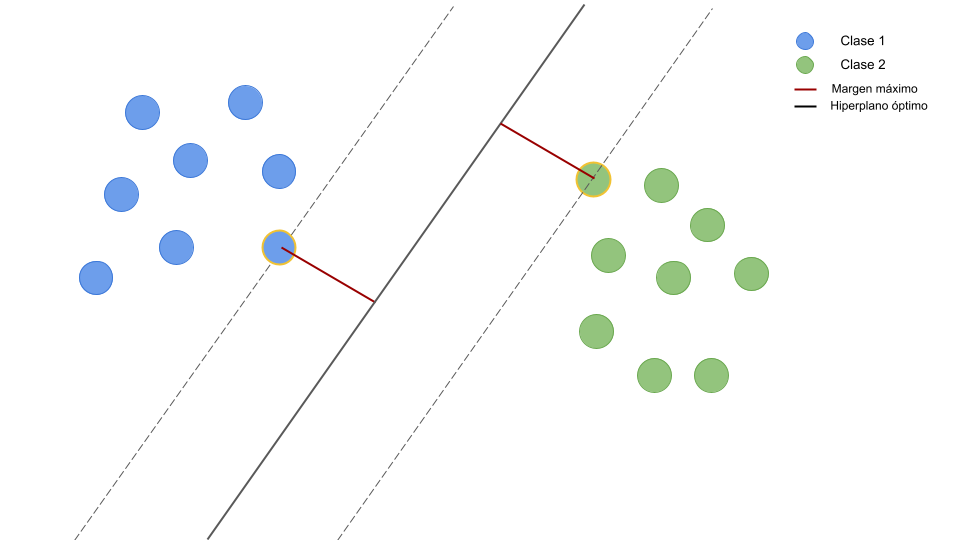
\includegraphics[width=10cm, keepaspectratio]{img/explicacion_svm.png}
  \caption{Ejemplo clasificación con Máquinas de soporte vectorial}\label{fig:explicacion_svm}
\end{figure}

En la Figura~\ref{fig:explicacion_svm} se puede ver un ejemplo de separación óptimo entre ambas clases, siendo los círculos rodeados en amarillo los vectores soporte. Ambos tienen la máxima distancia posible con el hiperplano generado, que es capaz de separar perfectamente ambas. El hiperplano de separación se puede definir como una función lineal:

\begin{equation}
    h(x) = \sum_{i= 0}^{n} w_i x_i
\end{equation}

Utilizando una vez más unos pesos ($w$) para encontrar dicho hiperplano.

Sin embargo, hay veces puede llegar a ser imposible hallar un hiperplano que divida correctamente las clases. Ante estos casos la resolución del problema se encuentra en aumentar la dimensionalidad de los datos para comprobar si en esa nueva dimensión existe un hiperplano capaz de separarlos adecuadamente.

Para implementar este tipo de modelo de aprendizaje en scikit-learn se puede utilizar la función SVC \cite{SVMDocumentation}. En esta ocasión este método no soporta multiprcesamiento, por lo tanto la máquina que lo ejecute solo podrá usar un core tanto en el entrenamiento como en la predicción.

\subsection{Gradient boosting}
\label{subsec:gradient_boosting}

Técnica de aprendizaje supervisado que se utiliza tanto para problemas de regresión como de clasificación. Se basa en la combinación de modelos predictivos débiles, normalmente árboles de decisión, para crear un modelo predictivo fuerte. Los árboles de decisión son uno de los algoritmos más utilizados para la toma de decisiones debido a su sencilla implementación y fácil interpretación. Dado un conjunto de datos se crean diagramas lógicos que sirven para representar una serie de condiciones sucesivas para resolver un problema. Por ejemplo en la Figura~\ref{fig:ejemplo_adecision} hay representado un árbol de decisión que sirve para poder saber si podemos salir a la calle a correr. 

\begin{figure}[h!]
  \centering
  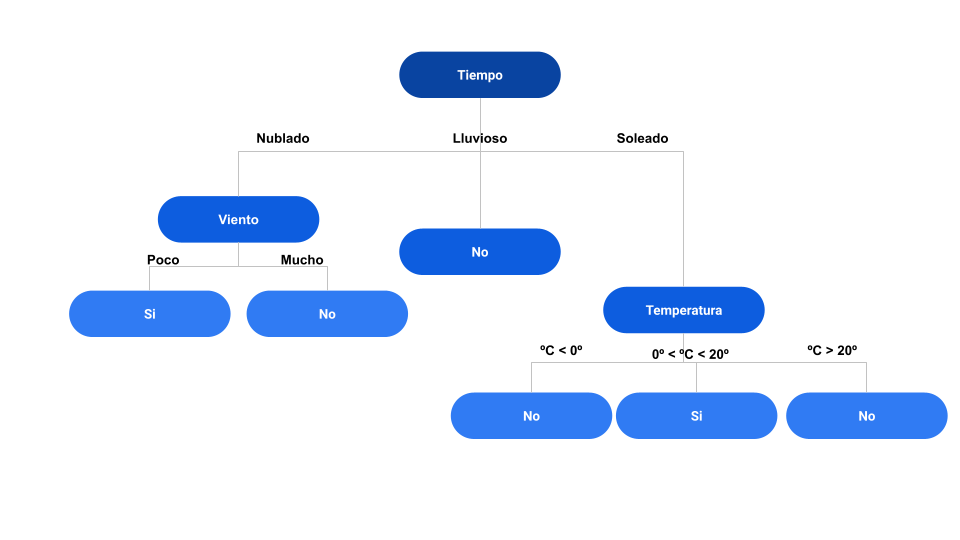
\includegraphics[width=14cm, keepaspectratio]{img/ejemplo_adecision.png}
  \caption{Ejemplo árbol de decisión.}\label{fig:ejemplo_adecision}
\end{figure}

En Gradient boosting se generan árboles de decisión de forma secuencial, haciendo que cada árbol corrija los errores del árbol anterior. De forma general suelen ser árboles de un máximo de tres niveles de profundidad.

En esta ocasión el método que crea este modelo es GradientBoostingClassifier\cite{GradientTreeBDoc}, que se encuentra dentro de la librería \textit{sklearn.esemble}. Al igual que para la función de máquinas de soporte vectorial, este modelo no soporta multiprocesamiento y por lo tanto solo se utilizará una cpu para entrenar y predecir con este modelo.

\subsection{Random forest}
\label{subsec:random_forest}

Random forest se puede usar tanto en problemas de clasificación como de regresión. Utiliza un conjunto de árboles de decisión con bagging, es decir, los árboles de decisión se generan de forma paralela. Al combinar sus resultados unos errores se compensan con otros, obteniendo una predicción que generaliza mejor.

En scikit-learn utilizando la función RandomForestClassifier\cite{RandomForestDoc}, que también está dentro de la librería \textit{sklearn.esemble}, se puede generar un modelo de aprendizaje utilizando esta técnica.

Para este método existe un parámetro destacable denominado \textit{n\_jobs}, que permite declarar el número de cpus que se desean utilizar para paralelizar el proceso. Para que se note el efecto de este parámetro es necesario que el conjunto de datos con el que se desea entrenar sea grande. De lo contrario el coste de distribuir los recursos entre el número de cores indicados es más elevado que ejecutarlo todo en una única cpu, y por lo tanto los tiempos de ejecución serían más elevados a mayor número definido en este parámetro.

Por defecto si no se declara este parámetro utilizará un único core. Además se pueden asignar valores negativos, en caso de igualar \textit{n\_jobs} a -1 se utilizarán todos los cores disponibles en ese momento. De la misma forma se utiliza este parámetro en el caso de Regresión logística cuando se busca entreanr un problemas de clasificación multiclase.

\section{DataSet: Room Occupacy}

Para realizar la clasificación en un inicio se utilizó el data set de Room Occupancy detection data\cite{DataSetOccupancy}, obtenido de Kaggle, que contiene unas 20560 muestras. Tal y como su nombre indica, este dataset proporcionará información sobre si una habitación se encuentra en un determinado instante ocupada o no. Cada ejemplo tiene las medidas de temperatura, humedad, CO2 y luz de una habitación de oficina de unos quince metros cuadrados. La última columna de cada fila indica la clase a la que pertenece la muestra. En este caso, al ser una clasificación binaria esta última columna solo puede tener dos valores, cero o uno. Si para un ejemplo contiene un uno significa que para esos valores sensados la habitación está ocupada. Si por el contrario hay un valor de cero la sala está vacia. 

Para generar los modelos se dividió el set de datos en dos partes, una primera parte para entrenar (que contenía el 70\% de ejemplos del set de datos original) y otra para comprobar la eficiencia del modelo a la hora de clasificar si la estancia está ocupada o no, un set de datos de prueba. En esta segunda parte se utilizó el 30\% restante de muestras del set de datos original, que no se utilizaban en el entrenamiento y por lo tanto el modelo nunca los había visto, son totalmente nuevos para él.

Un aspecto importante a destacar de este set de datos es que hay una mayor cantidad de ejemplos de habitación no ocupada que de ocupada. En otros sets de datos esto podría representar un problema ya que puede dar lugar a que al realizar esta división de forma aleatoria, el conjunto de datos de entrenamiento apenas tenga ejemplos de una de las clases. Sin embargo al tener una gran número de ejemplos en el que ambas clases tienen una gran cantidad de muestras, como es este caso, una división aleatoria no representa ningún inconveniente dado que hay una alta probabilidad de que el set de entrenamiento siempre tenga como mínimo la cantidad de muestras necesarias de ambas clases para entrenar correctamente. Aun así, la división se realizó de forma estratificada, para que hubiese la misma proporcion de datos de una clase u otra, que en el set de datos original. Y de esta forma nos aseguramos que a la hora de tanto entrenar, como de comprobar el modelo generado, se tengan ejemplos de ambas clases en la misma proporción que aparecen en el set de datos original.

Con esta división y preparación de los datos, los tres modelos se pudieron generar sin problemas utilizando las librerías de scikit-learn y pandas. Para valorar la eficiencia del entrenamiento se pueden utilizar tres valores diferentes: \textit{accuracy}, \textit{precision} y \textit{recall}. Gracias a la librería \textit{metrics} de scikit-learn se pueden obtener estos valores por medio de las funciones \textit{accuracy\_score}, \textit{precision\_score} y \textit{recall\_score} respectivamente. A estos métodos se les pasa como argumentos la variable que contiene los valores de la salida del set de datos de prueba (generada, como se ha comentado anteriormente, con el 30\% de los datos originales), y como segundo argumento el propio modelo generado (después de entrenarlo). 

A continuación se detalla que significan cada uno de esto valores. Para ello se ha definido la siguiente terminología: TP es el número de verdaderos positivos, TN verdaderos negativos, FP falsos positivos y FN falsos negativos.

El valor de \textit{accuracy} representa el porcentaje total de aciertos. Este dato se calcula por medio de la siguiente ecuación:

\begin{equation}
 \boxed{\mbox{Accuracy} = \frac{(TP + TN)}{(TP + TN + FP + FN)}}
\end{equation}

\textit{Precision} es el porcentaje que se obtiene al dividir el verdadero número de positivos (en este caso el valor positivo, o lo que es igual, el uno representa que la habitación está ocupada) entre todos los positivos que se han asignado (sean correctos o no). Cuanto más alto sea este valor menor error habrá cometido al asignar habitaciones ocupadas. DIcho valor viene dado por:

\begin{equation}
\label{eqn:accuracy} 
 \boxed{\mbox{Precision} = \frac{TP}{(TP + FP)}}
\end{equation}

Por último, para obtener el valor de \textit{recall} se dividen el número de verdaderos positivos entre la suma de los verdaderos positivos más los que son positivo y ha asignado como negativos. Siendo la fórmula por medio de la cual obtenemos este valor la siguiente:

\begin{equation}
 \boxed{\mbox{Recall} = \frac{TP}{(TP + FN)}}
\end{equation}

Todos conseguían un \textit{accuracy}, \textit{precision} y \textit{recall} superior al 90\%, el tiempo de ejecución era de un segundo para regresión logística, dos segundos tardaba el modelo de máquinas de soporte vectorial y gradient tree boosting y random forest eran los que más tardaban con un tiempo de cuatro y tres segundos respectivamente.

\subsection{Validación cruzada}

Se añadió un poco más de dificultad a la Raspberry haciendo que los algoritmos utilizasen validación cruzada, es decir, que dentro del set de datos de entrenamiento (compuesto, una vez más, por el 70\% de ejemplos del set de datos original) se hace una subdivisión en otros cinco sets para entrenar y probar el modelo con cada uno de ellos. 
Una vez realizada la validación cruzada se vuelve a probar la eficiencia del modelo haciendo que clasifique el 30\% de datos de la división original, son datos que nunca ha visto ni entrenado con ellos. El objetivo de realizar una validacion cruzada es garantizar que los resultados que obtengamos sean independientes de la partición entre datos de entrenamiento y datos de validación. Los resultados de esta prueba siguieron siendo muy buenos (el acierto seguía estando por encima del 90\%). 
En cuanto a los tiempos de ejecución el modelo de regresión logística incrementó el tiempo de ejecución siendo de cinco segundos. Para el modelo de máquinas de soporte vectorial el tiempo es de seis segundos. Random forest tarda en entrenar unos doce segundos. Y por último, el que más tiempo tarda es gradient tree boosting con un tiempo de diez y seis segundos. 


\section{DataSet: KddCup99}
\label{subsec:dataset_kddcup99}

Al realizar algunas pruebas para comprobar el comportamiento de la Raspberry ante diferentes situaciones de estrés (tal y como se explicará más adelante) los resultados obtenidos no encajaban del todo con lo esperado. Luego para tratar de comprender mejor lo que estaba pasando se decidió usar un dataset más grande que el anterior.

El dataset elegido fue KDD Cup 1999 Datadata\cite{DataSetOccupancy}, obtenido una vez más desde la página web de Kaggle. Se utilizó tanto el fichero \textit{kddcup.data.gz} como \textit{kddcup.data\_10\_percent.gz}. Una vez descargados se descomprimen y se ejecuta un programa para tratar los datos que contienen y poder utilizarlos en la generación de los modelos de Machine Learning.

Al igual que en el dataSet de Room Occupancy para la generación de los modelos se utilizará el 70\% de los datos para entrenar y el 30\% para validar.

\subsection{Preprocesamiento de kddCup99: prepare\_kddcup.ipynb}

Este fichero permite leer las líneas de los dataSet descargados, procesar y guardar los datos en un nuevo fichero para que puedan usarlos los modelos.

Para leer los datos se utiliza la función \textit{read\_csv} de pandas. Este programa no solo se usará para leer un dataSet al completo, sino que también podremos leer otra porción diferente de líneas. Es por esto que para que el programa ejecute correctamente hay que pasarle un número como único argumento, cuyo valor puede estar entre cero o cien. Este valor representa el porcentaje de datos que se desea leer. Un ejemplo de ejecución de este fichero para que lea el 50\% de los datos de kddCup99 es:\\

\begin{lstlisting}[language=bash]
    $ ipython Prepare_kddcup.ipynb 50
\end{lstlisting}

En el caso de \textit{kddcup.data} (que contiene más de un millón de líneas) interesa poder leer diferentes cantidades de datos del fichero puesto que tanto la Raspberry como el portátil no son capaces de leer este dataSet completo, los procesos morían antes de terminar. En el caso de la Raspberry el máximo de datos que es capaz de leer, sin que muera el proceso, es el cuarenta porciento del dataSet total mientras que el portátil llegaba al cincuenta porciento del total.

Para leer otro porcentaje del dataSet total, que no fuese únicamente el diez porciento, se utiliza una regla de tres. Sabiendo que el diez porciento del data set (el fichero \textit{kddcup.data\_10\_percent}) contenía 494020 líneas, se podía obtener aproximadamente tanto a cuantas líneas equivaldría otro porcentaje como la cantidad total de líneas que debía tener el dataSet completo.

La función \textit{random.sample} devuelve una lista que contiene valores numéricos aleatorios, para realizar esta función necesita que se le pasen dos argumentos. El primero de ellos es el valor máximo que puede aparecer en la lista, siendo el mínimo igual a cero. El segundo argumento es la longitud total de la lista, es decir, cuántos números aleatorios va a generar. Con este método se obtendrá una lista con valores aleatorios que se le asignará al parámetro skiprows de \textit{read\_csv}. Haciendo que todos esos datos, que representan números de líneas del fichero original, no se lean, consiguiendo hacer que se lea únicamente el porcentaje que ha pedido el usuario.

La implementación de esto se puede ver en el Código~\ref{lst:prepare_kddcup}, donde \textit{total} es el valor máximo de líneas que hay en el fichero \textit{kddcup.data} (obtenido mediante la regla de tres comentado anteriormente), \textit{per\_lines} es el número de líneas que sí se desean leer (obtenido al aplicar una regla de tres al porcentaje que se ha pasado como argumento a \textit{prepare\_kddcup.ipynb}). Ambos valores los usa \textit{random.sample} para obtener líneas aleatorias, que se ordenarán utilizando \textit{sorted} para poder pasárselas a skiprows y por lo tanto no se leerán. 

\begin{listing}[h!]
    \caption{Lectura del dataset y conversion a clase binaria.}{}
    \label{lst:prepare_kddcup}
    \begin{minted}[breaklines, fontsize=\footnotesize, baselinestretch=1]{python}
#Obtener número de lineas a leer
total= 4940200 # numero de lineas aproximado del fichero kddcup.data
per_lines= int((float(sys.argv[1])*total)/100)
#Leer dataSet
rm_lines= sorted(random.sample(range(total),total-per_lines))
dataset = pd.read_csv('/home/nuriadj/Documents/TFG/kdd_cup99/kddcup.data', skiprows=rm_lines)
print("Reading: %2.f" % round((len(dataset)*100)/total,2),"% of the csv")

#Conversión multiclase a binaria
dataset['normal.'] = dataset['normal.'].replace(['back.', 'buffer_overflow.', 'ftp_write.', 'guess_passwd.', 'imap.', 'ipsweep.', 'land.', 'loadmodule.', 'multihop.', 'neptune.', 'nmap.', 'perl.', 'phf.', 'pod.', 'portsweep.', 'rootkit.', 'satan.', 'smurf.', 'spy.', 'teardrop.', 'warezclient.', 'warezmaster.'], 'attack')
    \end{minted}
\end{listing}

Otro aspecto relevante que hay que saber acerca de este dataSet es que contiene datos que pertenecen a varias clases. Por lo tanto, dado que estamos resolviendo problemas de clasificación binaria, habrá que hacer un tratamiento previo a la información que contiene el dataSet para que se puedan agrupar los datos en dos clases en vez de en múltiples.\\
Este programa también hace esta conversión de multiclase a dos clases. Para ello, una vez leídos todos los datos se reemplazaban todas las clases (excepto la clase \textit{normal.}) por la clase \textit{attack}\cite{MulticlassToBinary}, de esta forma se conseguía tener solo dos clases. El código que realiza esta tarea se puede ver en Código~\ref{lst:prepare_kddcup}.

Una vez realizada la transformación de multiclase a clase binaria, se hace un pequeño tratamiento a los datos para que cada modelo pueda entrenar adecuadamente y más fácilmente con ellos\cite{dataSetTreatment}. Para ello se elimina la columna 19 y 20, ya que estas contienen todo el rato el mismo valor, que es cero. A continuación se transforman los datos categóricos y por último se eliminan las filas duplicadas. Con este tratamiento los datos se guardan utilizando la función \textit{to\_csv} que proporciona pandas y se guarda el nuevo set de datos tratados sin la cabecera ni el índice, de forma que desde el código de cada uno de los modelos los datos estén listos para poder ser utilizados.

\section{Dataset: Mi dataSet}
\label{sec:mi_dataSet}

A parte de los dataSets anteriores se creó uno a partir de la información recopilada por lo sensores mediante el programa \textit{read\_sensors.ipynb}. Este dataSet, con medidas de temperatura, humedad, presión y luz, busca generar un modelo que nos permita saber si la habitación está ocupada o no en un determinado instante, al igual que con el dataSet de Occupancy. 

Para ello durante quince minutos se estuvieron tomando las medidas en una habitación de forma controlada, es decir, sabiendo en cada instante si la habitación estaba ocupada o no. Durante diferentes periodos de tiempo la habitación estuvo ocupada o vacía. Cuando la habitación estaba vacía algunas veces se cerraba la persiana de la habitación para que también tomase medidas bajo esta nueva condición.

Una vez finalizado el tiempo que se deseaba hacer la prueba se paraba el programa \textit{read\_sensors.ipynb}, se abría el nuevo csv generado y se añadia al csv una nueva columna que representa el estado de la habitación en cada instante, asignando un uno cuando estaba ocupada y un cero en el caso contrario.

\subsection{read\_sensors.ipynb}
\label{subsec_read_sensors}

Como se ha comentado anteriormente este programa es el encargado de tomar las medidas de los sensores conectados a la Raspberry, guardarlas y generar con ellas un nuevo csv y una imagen, que muestra de forma gráfica los valores sensados en cada instante de tiempo para que visualmente sea más fácil interpretar lo que ha pasado en ese periodo de tiempo. 

Para que pueda ejecutar correctamente es necesario que se le pase como argumento el nombre con el que se desea guardar el dataSet que se va a generar. Este argumento también se utilizará para nombrar la gráfica que genera el programa con el siguiente formato: \textit{Dara\_graph\_miDataSet}, siendo miDataSet el string que se haya pasado como argumento.

Este programa necesita usar la comunicación I2C para obtener los valores del sensor BME280 pero también necesitará acceder directamente a los pines por medio de la librería LGPIO. Para poder utilizar LGPIO es necesario ejecutar el programa con permisos de root pero manteniendo el entorno conda actual (pues es donde se encuentran todas las librerías instalaldas), es por ello que para ejecutarlo habrá que utilizar la siguiente línea de comando:  


\begin{lstlisting}[language=bash]
    $ sudo env "PATH=$PATH" ipython read_sensors.ipynb miDataSet
\end{lstlisting}

Una vez ejecutado el programa, en la segunda celda de este, se preprararán los puertos para poder leer los datos. 

A continuación se quedará ejecutando indefinidamente un bucle while, que es el que se encarga de guardar los datos sensados cada un segundo. Dicho bucle se puede ver en el Código~\ref{lst:firstloop_read_sensor}. Algo destacable es que al valor de la luz (proporcionada por el LDR) siempre se le resta uno. Esto se hace así para que los datos se puedan interpretar mejor, puesto que cuando hay luz a la Raspberry le llega un cero. De esta forma cuando haya luz se guarda un uno en el fichero en vez de un cero. 
Este bucle estará continuamente mostrando por el terminal las medidas tomadas hasta que el usuario haga Ctr-C , de esta forma se indica que ya no se desean guardar más datos.

\begin{listing}[h!]
    \caption{Bucle que guarda los datos sensados.}{}
    \label{lst:firstloop_read_sensor}
    \begin{minted}[breaklines, fontsize=\footnotesize, baselinestretch=1]{python}
measures= [] #array que contiene los valores del sensor

try:
    while True:

        bme280_data = bme280.sample(bus, address)
        humidity= bme280_data.humidity
        pressure= bme280_data.pressure
        temp= bme280_data.temperature
        
        light= lgpio.gpio_read(h, LDR)
        light= 1 - light
        
        measures.append([humidity, pressure, temp, light])
        
        print(humidity, pressure, temp, light)
        time.sleep(1)
except KeyboardInterrupt:
   pass  
    \end{minted}
\end{listing}

Una vez que este bucle ha finalizado, se ejecuta otro que iterará sobre los datos guardados en la lista \textit{measures} para poder pintar esos valores en la gráfica que devuelve este programa. Dicho bucle se puede ver en el segmento de Código~\ref{lst:secondloop_read_sensor}. Hay dos cosas destacables de este trozo de código. La primera es que el valor de las presiones se divide entre diez. Esto se debe a que las presiones que devuelve el sensor BME280 son valores muy superiores a los que puede conseguir cualquiera de los otros sensores, por lo que en vez de devolver la medida en $hPa$ se divide entre diez para obtenerla en $KPa$ y de esta forma poder apreciar mejor los cambios sensados en todos los sensores.


El segundo aspecto destacable es sobre el valor de la luz, que se multiplica por cincuenta. Al igual que en el caso de las presiones esto se hace para que el cambio de estado entre oscuridad y luz sea apreciable en la gráfica, de lo contrario el salto entre ceros y unos apenas se podrían ver.

\begin{listing}[h!]
    \caption{Bucle para generar la gráfica.}{}
    \label{lst:secondloop_read_sensor}
    \begin{minted}[breaklines, fontsize=\footnotesize, baselinestretch=1]{python}
hum= []
temp= []
pres= []
light= []
x= []

for i in range(len(measures)):
    hum.append(measures[i][0])
    pres.append(measures[i][1]/10)
    temp.append(measures[i][2])
    light.append((measures[i][3]*50))#multiplico por 50 para verlo mejor en el plot
    x.append(i)
    \end{minted}
\end{listing}

Un ejemplo de la gráfica que genera este programa se puede observar en la Figura~\ref{fig:ejemplo_gráfica}. Donde el eje x representan los minutos que han pasado desde que comenzó a ejecutarse el código.

\begin{figure}[h!]
  \centering
  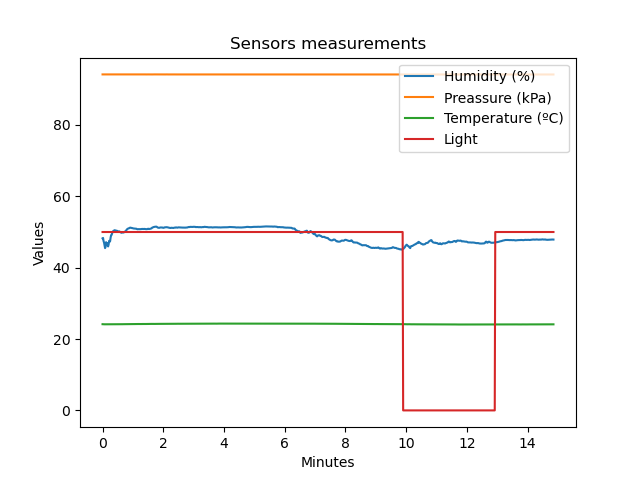
\includegraphics[width=11cm, keepaspectratio]{img/occup_detec_15m.png}
  \caption{Ejemplo gráfica de las medidas de los sensores.}\label{fig:ejemplo_gráfica}
\end{figure}

\cleardoublepage

%%%%%%%%%%%%%%%%%%%%%%%%%%%%%%%%%%%%%%%%%%%%%%%%%%%%%%%%%%%%%%%%%%%%%%%%%%%%%%%%
%%%%%%%%%%%%%%%%%%%%%%%%%%%%%%%%%%%%%%%%%%%%%%%%%%%%%%%%%%%%%%%%%%%%%%%%%%%%%%%%
% EXPERIMENTOS Y VALIDACIÓN %
%%%%%%%%%%%%%%%%%%%%%%%%%%%%%%%%%%%%%%%%%%%%%%%%%%%%%%%%%%%%%%%%%%%%%%%%%%%%%%%%

\chapter{Experimentos y validación}
\label{chap:experimentos}

\textbf{Atención}: Este capítulo se introdujo como requisito en 2019.

\begin{comment}
Describe los experimentos y casos de test que tuviste que implementar para validar tus resultados. 
Incluye también los resultados de validación que permiten afirmar que tus resultados son correctos.
\end{comment}

En este capítulo comprobaremos la eficiencia de la Raspberry a la hora de generar los modelos comentados en el capítulo anterior para que se ajusten al dataSet kdd\_cup99 comentado anteriormente. Las pruebas consistirán en someter a la máquina a diferentes niveles de cargas computacionales para observar como lidia la Raspberry con la generación del modelo a la vez que con estas cargas.
Además nos ayudaremos de un portátil para poder comparar los resultados de ambos dispositivos.

\section{Experimentos en la Raspberry}
\label{sec:experimentos_en_raspberry}

Para comprobar la capacidad de la Raspberry para generar estos modelos se definieron cuatro niveles de saturación: el nivel "Idle" en el que no se somete a la máquina a ningún tipo de carga extra, el nivel bajo, que consistía en estresar una única cpu, el nivel medio, dos cpus y por último en el nivel alto se estrasaban todas las cpus de la Raspberry, es decir, cuatro cpus. 
Para estresar las cpus se utilizó el comando \textit{stress} que permite estresar, durante el tiempo que se le indique, el número de cpus que se comanden.

Luego cada uno de los modelos se sometía a estos cuatro niveles de carga. La medida que se utiliza para comparar los diferentes niveles es el tiempo que tarda cada uno de los modelos en terminar de ejecutar. Para obtener dicho tiempo se utiliza el comando \textit{time} de Linux, con el que se ejecutaba cada modelo de la siguiente forma:\\

\begin{lstlisting}[language=bash]
  $ time ipython modelo.ipynb
\end{lstlisting}

El comando \textit{time} devuelve tres valores. Uno de ellos es el tiempo de usuario, que es la cantidad de tiempo que se ha gastado el proceso en modo usuario. El Sys time es el tiempo de CPU invertido en el kernel dentro del proceso. Con estos dos tiempos se puede obtener el Cpu time, el tiempo total que ha utilizado la CPU para completar la ejecución del proceso. Por otra parte time también proporciona el real time, el tiempo que ha tardado en ejecutar el proceso como si lo hubiesemos cronometrado con un reloj, este tiempo es igual que el Wall time. Es necesario entender esto para poder comprender los valores que nos devolverán los experimentos.

En caso de querer someter a la Raspberry a un nivel mayor de carga computacional se ejecutaban paralelamente el comando \textit{stress} y el modelo.


\subsection{Programa para las pruebas: raspberry\_test.ipynb}
\label{subsec:programa_pruebas_raspberry}

Para realizar las pruebas en la Raspberry de forma más sencilla se creó un programa llamado \textit{raspberry\_test.ipynb}. Dicho programa necesita como único argumento el data set con el que se desea hacer el experimento para que pueda realizar su función correctamente.

Hay que tener en cuenta que si se quiere usar este código, el dataSet que se quiera utilizar para entrenar debe de estar limpio, es decir, se le ha hecho un preprocesamiento para borrar características no deseadas o redundantes. Tampoco debe de tener cabecera. Si no se hace este preprocesamiento podrá dar error la ejecución.

La misión de este código es ejecutar cada uno de los modelos de aprendizaje automático (que se utilizan en este proyecto) con los diferentes niveles de saturación comentados anteriormente. Para realizar esto se usan dos bucles anidados, el primero de ellos itera sobre los modelos que se desean poner a prueba. El segundo recorre una lista que contiene el número de cores que se desean estresar con cada uno de los modelos (ver código ~\ref{lst:funcion_principal_raspberry_test}). Si el valor sobre el que se está iterando de la lista es mayor que cero significa que se desea estresar cierto número de cpus, por lo tanto se llama a la función \textit{start\_stress} a la que se le pasa como argumento el número de cores a estresar y durante cuanto tiempo, con estos datos se encargará de crear un nuevo proceso para ejecutar el comando \textit{stress}.\\
Por otra parte, independientemente del número de cores, siempre se llamará a la función \textit{model} que creará un nuevo proceso para ejecutar, utilizando el comando \textit{time} de Linux, uno de los ficheros que se encuentran dentro de la carpeta \textit{"Modelos"}. Cada uno de los ficheros que se encuentran dentro de dicha carpeta generará uno de los modelos de aprendizaje automático que se han explicado en este proyecto. 

\begin{listing}[h!]
    \caption{Función principal raspberry\_test.ipynb}{}
    \label{lst:funcion_principal_raspberry_test}
    \begin{minted}[breaklines, fontsize=\footnotesize, baselinestretch=1]{python}
#Hacer una version que ejecute de seguido los modelos solo (sin stress)
t= 200
list_cpus= [0,1,2,4]
dataSet= sys.argv[1]
name_dataSet= dataSet.split("/")[-1].split(".csv")[0]

lst_header= []
lst_Wt= []
lst_Ct= []
lst_TAc= []
lst_Ac= []
lst_Pr= []
lst_Re= []

for i in range(4):
    for j in list_cpus:
        num_cores= j
        
        if(j > 0):
            pid_stress= start_stress(j, t)
        else:
            print("\nCpu Idle")
            
        model_num= i    
        model(model_num)
        
        if j > 0:
            os.killpg(os.getpgid(pid_stress.pid), signal.SIGKILL)
        
        print("Sleeping for 5 sec...\n")
        time.sleep(5)
    \end{minted}
\end{listing}

Cuando se completa la generación del modelo para uno de los niveles, los resultados de Cpu time, Wall time, Accuracy trainning (que es el valor de Accuracy para los mismos datos con los que se ha entrenado), Accuracy, Presisión y Recall se van guardando cada uno en su respectiva lista gracias a una función del programa llamada \textit{get\_data}. Una vez que uno de los modelos ha completado todas las pruebas se genera una tabla mediante la función \textit{add\_data} con los resultados obtenidos en cada uno de los casos.
Dicha tabla se guardará en un fichero que se encarga de crear \textit{raspberry\_test.ipynb}. Este fichero tendrá por nombre el siguiente formato: nombreDataSet\_raspMD.csv, donde MD son las siglas del modelo que se ha ejecutado. Por ejemplo, en el caso de Regresión logísitca el nombre será nombreDataSet\_raspRL.csv, o en el caso de Máquinas de soporte vectorial nombreDataSet\_raspSVM.csv. En total el programa creará cuatro csv diferentes, un por cada modelo

Los nuevos procesos, comentados anteriormente, se crean utilizando la función \textit{Popen} de la librería \textit{subprocess}. Nótese que en el método \textit{model} (a diferencia de \textit{start\_stress}) esta función tiene añadido al final un \textit{.communicate()} de esta forma se parará la ejecución principal hasta que el proceso de \textit{Popen} termine. Si una vez terminado dicho proceso \textit{stress} sigue ejecutando se matará para poder comandar otro \textit{stress} sin tener que esperar a que se cumpla el tiempo de ejecución que le pasamos como argumento como se puede ver en el Código~\ref{lst:funcion_principal_raspberry_test}.


\subsection{Resultados Occupancy}
\label{subsec:resultados_raspberry}

\subsection{Resultados kdd\_cup99}
\label{subsec:resultados_raspberry}

Los resultados obtenidos para el veinte por ciento del data set de Kdd\_cup99 son los siguientes: 

\definecolor{myGray}{rgb}{0.9, 0.9, 0.9}
\begin{table}[H]
\begin{adjustbox}{width=\textwidth}
\renewcommand{\arraystretch}{2}
\newcolumntype{a}{>{\columncolor{lightgray}}c}
\centering
    \begin{tabular}{ | a | c | c | c | c | c | c | c | c |}
    \hline
    \rowcolor{lightgray}\multirow{2}{*}{\textbf{Modelo}} & \multicolumn{2}{|c|}{\textbf{Idle}} & \multicolumn{2}{|c|}{\textbf{1 cpu}} & \multicolumn{2}{|c|}{\textbf{2 cpu}} & \multicolumn{2}{|c|}{\textbf{4 cp}}\\[2ex]
    \cline{2-9}
     & \cellcolor{myGray}Cpu time & \cellcolor{myGray}Wall time & \cellcolor{myGray}Cpu time & \cellcolor{myGray}Wall time & \cellcolor{myGray}Cpu time & \cellcolor{myGray}Wall time & \cellcolor{myGray}Cpu time & \cellcolor{myGray}Wall time\\[2ex]
    \hline
    Regresión logísitca & 1 min 36 seg & 38 seg & 1 min 48 seg & 50 seg & 1 min 33 seg & 56 seg & 1 min 34 seg & 57 seg \\[2ex]
    \hline
    SVM & 2 min 19 seg & 2 min 16 seg & 2 min 17 seg & 2 min 18 seg & 2 min 12 seg & 2 min 12 seg & 2 min 18 seg & 2 min 18 seg\\[2ex]
    \hline
    Gradient boosting & 3 min 19 seg & 3 min 20 seg & 3 min 19 seg & 3 min 20 seg & 3 min 15 seg & 3 min 15 seg & 3 min 16 seg & 3 min 17 seg\\[2ex]
    \hline
    Random forest & 3 min 4 seg & 1 min 3 seg & 2 min 30 seg & 1 min 5 seg & 2 min 3 seg & 1 min 10 seg & 2 min 10 seg & 1 min 18 seg\\[2ex]
    \hline
    \end{tabular}
\end{adjustbox}
\caption{Tiempos de generación de los modelos en Raspberry para diferentes niveles de saturación}
\label{tab:times_raspberry}
\end{table}

Como se puede observar en la tabla anterior, los tiempos varian entre los diferentes modelos, siendo el de Regresión logística el que menos tiempo tarda en todos los casos.

Un aspecto destacable es que los tiempos de Regresión logísitca, Máquinas de soporte vectorial (SVM) y Gradient boosting apenas varían entre los diferentes niveles de estrés. En el caso de Máquinas de soporte vectorial y Gradient boosting esto se debe a que scikit-learn no admite multi-threading, por lo que a pesar de estresar una, dos o cuatro cpus siempre devolverán el mismo tiempo puesto que estos modelos solo pueden utilizar un único core para ejecutar.\\
Regresión logística podría utilizar varios cores si se le indica mediante el parámetro n\_jobs. Pero dado que estamos en un problema de clasificación binaria este valor no tendrá ningún efecto al aumentar o disminuir el número de cpus estresadas como vimos en el apartado~\ref{subsec:regresion_logistica}.

En cuanto al modelo de Random forest, para poder entender los tiempos que devuelve, es necesario explicar primero como se comporta la Raspberry cuando varios procesos le piden más recursos de los que tiene y como afecta el parámetro n\_jobs a los tiempo de este modelo.

Comencemos explicando como afecta el parámetro n\_jobs a los tiempos de ejecución. Como se ha visto anteriormente, Random forest admite el parámetro n\_jobs, que en este caso (a diferencia de Regresión logística) sí que afecta a como ejecuta el modelo independientemente de si es un problema de clasificación binaria o no. Por lo tanto para poder optimizar el proceso habrá que hacer que el parámetro n\_jobs sea igual al número de cores del dispositivo, que en este caso serán cuatro. 

Con este parámetro ajustado hay que saber que el tiempo de Cpu que obtenemos del comando time es la suma de los tiempos que ha necesitado cada uno de los cores utilizados por el proceso para la ejecución. Esta es la razón por la que podemos ver como el tiempo en Idle es bastante mayor que el resto de casos, puesto que es en esta ocasión donde el programa está pudiendo hacer un uso completo de los cuatro cores, ya que no hay ningún otro proceso que necesite usarlos. Por lo tanto el Cpu time que tenemos en este nivel es en realidad la suma de los tiempos de ejecución de los cuatro cores. El tiempo que ha necesitado cada uno de los cores sería dividir 3min 4seg entre 4 con lo que obtendríamos 46 segundos por core. Sabiendo esto queda explicado por qué el nivel de Idle devuelve un valor tan alto y como esto, que a prioir puede parecer un poco contradictorio, se ajusta a lo esperado.

Para el resto de casos, dado que ya intervienen otros procesos, habrá que saber como se comporta la Raspberry ante una mayor demanda de recursos. Lo primero que hay que saber es que el comando \textit{stress} estresará el número de cpus que se le pasan como argumento siempre y cuando pueda. En el momento en el que tenga que compartir Cpu con otros procesos, la Raspberry repartirá los recursos haciendo que \textit{stress} no utilice todas las cpus que se le ha comandado estresar para que el otro proceso también pueda ejecutar. Por ejemplo, cuando se realiza la prueba de nivel alto al modelo de Máquinas de soporte vectorial, si se comprueban los valores de cpu que utiliza cada uno de los procesos (por medio del comando htop de Linux), a pesar de que stress tiene cuatro procesos la suma de lo que utiliza la cpu cada uno de ellos será igual a un total de tres cores más o menos, es decir utilizan un 300\% de los recursos. Mientras que el proceso del modelo utiliza una cpu, un 100\%. Siendo el valor total de los recursos de los que dispone la Raspberry igual a 400\%, un 100\% para cada uno de los cores de la Raspberry.

Otro ejemplo de esto puede ser el caso en el que se ejecuta Random forest, teniendo el parámetro de n\_jobs igual a cuatro para utilizar todos los cores disponibles, a la vez que stress para estresar las cuatro cpus. Si observamos mediante el comando htop los procesos, se podrá ver como se distribuyen los cores para que puedan ejecutar a la vez tanto los procesos de stress como los del modelo de aprendizaje. Por lo tanto stress utilizará en total dos cpus y Random forest hará lo mismo, a pesar de que a ambos se les indicó que utilizasen todas las cpus de la Raspberry. Este ejemplo se puede ver en la figura~\ref{figura:stress_rForest}.\\

 \begin{figure}[H]
    \centering
    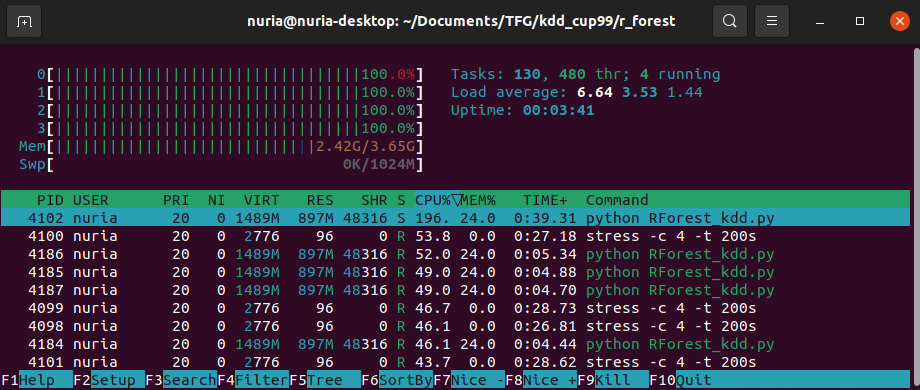
\includegraphics[ width=16cm, keepaspectratio]{img/rFores_stress.png}
    \caption{Ejecución Random forest con cuatro cpus estresadas}
    \label{figura:stress_rForest}
 \end{figure}

En la figura~\ref{figura:stress_rForest} vemos que el proceso de Random forest está consumiendo el 196\% de cpu, prácticamente un 200\%. Mientras que si sumamos los porcentajes de los cuatro procesos de \textit{stress} obtendremos que se están consumiento en total un 190\%. Por lo que a pesar de lo que se ha comandado, la Raspberry dividirá los recursos para que ambos procesos puedan usar lo máximo posible.

Sabiendo esto, los niveles de prueba medio y alto obtienen prácticamente los mismos tiempos puesto que al tratar de ejecutar a al vez tanto el proceso de stress como el del modelo se están pidiendo usar más cores de los que hay. En consecuencia la Raspberry tendrá que dividir los recursos de los que dispone equitativamente entre ambos procesos. Por lo que en el fondo stress estará estresando el mismo número de cpus tanto en el nivel medio como en el alto y al proceso del modelo le sucederá lo mismo, utilizará el mismo número de cores tanto en un caso como en el otro. En el nivel intemedio, donde se estresan dos cores, el modelo no podrá utilizar las cuatro cpus que se le indican con n\_jobs puesto que estaría superando el número de cores que tiene la Raspberry. De modo que la Raspberry dividirá los recursos haciendo que stress pueda ejecutar en dos cores, y por lo tanto el modelo de aprendizaje dispondrá únicamente de las otras dos cpus para su ejecución. Mientras que en el nivel más alto de carga la Raspberry dividirá las cuatro cpus para darle la mitad de ellas a la ejecución de \textit{stress} y la otra mitad al modelo, haciendo que ambas utilicen el máximo de cores posibles.

Otro aspecto de las ejecuciónes en la Raspberry  que será relevante más adelante, es la frecuencia a la que ejecutan los core. Utilizando el comando \textit{lscpu} de Linux, se puede obtener información relevante sobre los cores como por ejemplo la frecuencia máxima y mínima a la que pueden ejecutar, que en el caso de la Raspberry la mínima será igual a 600MHz y la máxima 1500MHz. 

Para saber la frecuencia de cada uno de los cores en tiempo real se puede ejecutar el comando:\\

\begin{lstlisting}[language=bash, showstringspaces=false]
   $ watch -n.1 "
   sudo cat /sys/devices/system/cpu/cpu0/cpufreq/cpuinfo_cur_freq && 
   sudo cat /sys/devices/system/cpu/cpu1/cpufreq/cpuinfo_cur_freq && 
   sudo cat /sys/devices/system/cpu/cpu2/cpufreq/cpuinfo_cur_freq && 
   sudo cat /sys/devices/system/cpu/cpu3/cpufreq/cpuinfo_cur_freq"
\end{lstlisting}

Mostrará las frecuencias de ejecución de los cores cada 0.1 segundos. Si utilizamos dicho comando para ver las frecuencias cuando la Raspberry está tanto Idle como estresada podremos ver que todas las cpus están sobre los 1500MHz. Por lo tanto todos los cores siempre están ejecutando a la máxima velocidad que pueden.

\section{Experimentos en el portátil}
\label{sec:experimentos_en_portatil}

Las mismas pruebas que se realizaron en la Raspberry se llevaron a cabo en un portátil. De esta forma se podrán comparar los tiempos de ejecución en un dispositivo de mayor capacidad y sabremos cuanto dista el comportamiento de la Raspberry del de una máquina con mayor potencia.

El portátil que se utilizó para estas pruebas tenía un total de ocho cpus físicas. Es por ello que, salvo el nivel Idle, los cores de los niveles bajo, medio y alto de carga computacional cambiaron para poner más o menos en la misma situación al portátil y a la Raspberry. Por lo tanto en el portátil el nivel bajo de carga será estresar dos de sus cpus, el nivel medio cuatro y el alto los ocho cores de los que dispone la máquina. 

\subsection{Programa para las pruebas: pc\_test.ipynb}
\label{subsec:programa_pruebas_pc}

Para realizar las pruebas se ha creado un programa llamado \textit{pc\_test.ipynb} que al igual que el fichero \textit{raspberry\_test.ipynb} ejecuta cada uno de los modelos con los diferentes niveles de estrés y guarda los datos obtenidos en un nuevo fichero que crea el programa con el formato nombreDataSet\_pcMD.csv, siendo MD una vez más las siglas del modelo de aprendizaje automático. El programa generará un fichero diferente para cada modelo.

Al igual que en \textit{raspberry\_test.ipynb} el dataSet que se quiera utilizar para entrenar debe de haber sido preprocesado (en caso de que lo necesite) y no debe de tener cabecera, sino dará error la ejecución.

La función principal utilizará dos bucles anidados, tal y como se hacia en \textit{raspberry\_test.ipynb}, para iterar sobre los modelos de aprendizaje con los que se desean experimentar y el número de cores que se van a estresar en cada prueba. En este caso la lista denominada como \textit{num\_cores} variará respecto a la que se declaró en \textit{raspberry\_test.ipynb} ya que como se ha comentado antes, en esta ocasión tendremos que saturar otras cantidades de cores. Este programa creará (si es necesario) dos procesos, uno ejecutará stress (cuando se desee estresar alguna cpu) y el otro los modelos que se encuentran dentro de la carpeta \textit{"Modelos"}. Todos los ficheros que generan los modelos de aprendizaje son los mismos que en la Raspberry salvo el de Random Forest que tiene un fichero específico para el portátil puesto que en este caso, el parámetro \textit{n\_jobs} tendrá que ser igual a ocho, para que el modelo pueda disponer de todos los cores que tiene el portátil. 

\subsection{Resultados kdd\_cup99}
\label{subsec:resultados_pc}

Los resultados de la ejecución del comando stress conforme a estos niveles se pueden observar en la tabla~\ref{tab:times_portatil}. Como se puede apreciar los tiempos que se obtienen en el portátil disminuyen bastante con respecto a los que conseguía la Raspberry. 

\definecolor{myGray}{rgb}{0.9, 0.9, 0.9}
\begin{table}[h!]
\begin{adjustbox}{width=\textwidth}
\renewcommand{\arraystretch}{2}
\newcolumntype{a}{>{\columncolor{lightgray}}c}
\centering
    \begin{tabular}{ | a | c | c | c | c | c | c | c | c |}
    \hline
    \rowcolor{lightgray}\multirow{2}{*}{\textbf{Modelo}} & \multicolumn{2}{|c|}{\textbf{Idle}} & \multicolumn{2}{|c|}{\textbf{2 cpu}} & \multicolumn{2}{|c|}{\textbf{4 cpu}} & \multicolumn{2}{|c|}{\textbf{8 cp}}\\[2ex]
    \cline{2-9}
     & \cellcolor{myGray}Cpu time & \cellcolor{myGray}Wall time & \cellcolor{myGray}Cpu time & \cellcolor{myGray}Wall time & \cellcolor{myGray}Cpu time & \cellcolor{myGray}Wall time & \cellcolor{myGray}Cpu time & \cellcolor{myGray}Wall time\\[2ex]
    \hline
    Regresión logísitca & 18 seg & 7 seg & 21 seg & 8 seg & 29 seg & 13 seg & 48 seg & 27 seg \\[2ex]
    \hline
    SVM & 31 seg & 31 seg & 43 seg & 43 seg & 58 seg & 58 seg & 1 min 22 seg & 1 min 32 seg\\[2ex]
    \hline
    Gradient boosting & 41 seg & 41 seg & 54 seg & 54 seg & 1 min 27 seg & 1 min 27 seg & 1 min 29 seg & 1 min 41 seg\\[2ex]
    \hline
    Random forest & 1 min 16 seg & 13 seg & 1 min 5 seg & 15 seg & 58 seg & 19 seg & 54 seg & 23 seg\\[2ex]
    \hline
    \end{tabular}
\end{adjustbox}
\caption{Tiempos de generación de los modelos en el portátil para diferentes niveles de saturación}
\label{tab:times_portatil}
\end{table}

Como se puede ver Random Forest es el modelo que más tiempo tarda cuando la máquina se encuentra en estado Idle. Esto se debe a las mismas razones dadas en la sección~\ref{subsec:resultados_raspberry}

Otro aspecto destacable de los tiempos en el portátil es que estos aumentaban a medida que se estresaba un mayor número de cores a pesar de que los tres primeros procesos siguen siendo monocores. Esto se debe a la frecuencia con la que ejecutan las cpus. En el portátil la frecuencia máxima a la que pueden ejecutar los cores es de 3600 MHz mientras que la mínima son 400 MHz. 

Ejecutando el siguiente comando: 

\begin{lstlisting}[language=bash, showstringspaces=false]
  $ watch -n.1 "grep \"^[c]pu MHz\" /proc/cpuinfo"
\end{lstlisting}

Se puede ver la frecuencia de ejecución de todos los cores cada 0.1 segundos. En esta ocasión al observar estas velocidades cuando se ejecutaban los algoritmos de aprendizaje automático se podía ver una variación en los valores dependiendo del nivel de estrés que se estuviese ejecutando. Luego esto explicaría porque en el caso del portátil los tiempos incrementan según aumentan el número de cores estresados. 

\section{Comparación Raspberry vs Portátil}
\label{sec:raspberry_vs_portatil}

Lo primero que puede llamar la atención de ambas tablas es que la Raspberry, para los mismos modelos y los mismos datos, tarda más en ejecutar que el portátil. Esto se debe a que habiendo observado las frecuencias tanto de la Raspberry como del portátil vemos que la máxima velocidad a la que pueden ir los cores en la Raspberry es a 1500 MHz mientras que el portátil tiene su máximo en 3600 MHz, más del doble que la Raspberry. Luego esto permite que los procesos en el portátil puedan terminar antes que en la Raspberry siendo uno de los factores por los que la Raspberry puede ser más lenta que el portátil, ya que los cores pueden ir a mayor velocidad.

Sin embargo, a parte de la diferencia de los tiempos, todos los modelos tanto entrenando en la Raspberry como en el portátil alcanzaban un Accuracy, Precision y Recall mayor al 90\% prácticamente siempre en todos los casos.
 
\section{Incorporación de código en la memoria}

Es bastante habitual que se reproduzcan fragmentos de código en la memoria de un TFG/TFM.
Esto permite explicar detalladamente partes del desarrollo que se ha realizado que se consideren
de especial interés. No obstante, tampoco es conveniente pasarse e incluir demasiado código en
la memoria, puesto que se puede alargar mucho el documento. Un recurso muy habitual es subir
todo el código a un repositorio de un servicio de control de versiones como GitHub o GitLab,
y luego incluir en la memoria la URL que enlace a dicho repositorio.

Para incluir fragmentos de código en un documento \LaTeX se pueden combinar varias
herramientas:

\begin{itemize}
    \item El entorno \mintinline{latex}{\begin{listing}[]...\end{listing}} permite crear
    un marco en el que situar el fragmento de código (parecido al generado cuando insertamos
    una tabla o una figura). Podemos insertar también una descripción (\textit{caption})
    y una etiqueta para referenciarlo luego en el texto.
    
    \item Dentro de este entorno, se puede utilizar el paquete 
    \mintinline{latex}{minted}~\footnote{\url{https://es.overleaf.com/learn/latex/Code_Highlighting_with_minted}},
    que utiliza el paquete Python Pygments para resaltado de sintaxis (coloreando el
    código). Como se puede ver en el siguiente ejemplo, hay muchas opciones de configuración
    que permiten controlar cómo se va a mostrar el código (incluir números de línea, saltos
    de línea, tamaño y tipo de fuente, espaciado, código de colores para resaltado, etc.).
\end{itemize}

\begin{listing}[h!]
    \caption{Lectura de un fichero *.csv y tipado de datos.}{}
    \label{lst:1}
    \begin{minted}[breaklines, fontsize=\footnotesize, baselinestretch=1]{python}
# A dictionary is built to define the data type contained by each column
dtype_scheme ={'budget': np.int64, 'genres': np.object, 'homepage': np.str, 'id': np.int64, 'keywords': np.object, 'original_language': np.str, 'original_title': np.str, 'overview': np.str, 'popularity': np.float64, 'production_companies': np.object, 'production_countries': np.object, 'release_date': np.object, 'revenue': np.int64, 'runtime': np.float64, 'spoken_languages': np.object,  'status': np.object, 'tagline': np.str, 'title': np.str, 'vote_average': np.float64, 'vote_count': np.int64}

# When loading the data from the .csv file, we provide the scheme to be followed for data typing
df1 = dd.read_csv('tmdb_5000_movies.csv', dtype=dtype_scheme)
    \end{minted}
\end{listing}

Otra ventaja del entorno \verb|listing| es que se puede generar automáticamente un índice
(con entradas hiperenlazadas) de fragmentos de código, para incluirlo al comienzo del 
documento junto con los índices de figuras, tablas, etc.

\subsection{Fuentes monoespaciadas}

A veces se incluyen nombres de archivos, paquetes, etc. como texto monoespaciado, utilizando
el comando \LaTeX \mintinline{latex}{\texttt{}}. Sin embargo, esto puede generar un problema
cuando las palabras en fuente monoespaciada alcanzan el final de una línea. En ese caso,
el compilador rehusa muchas veces romper la palabra y deja la línea demasiado larga respecto
al resto.

Para evitar esto, especialmente en párrafos más cortos de lo habitual (como en una lista
no numerada), se puede utilizar el comando \mintinline{latex}{\begin{sloppypar}...\end{sloppypar}},
como se muestra a continuación con un ejemplo real.
    
\begin{itemize}
    
    \begin{sloppypar} % Arregla longitud de línea en párrafos con fuente monoespaciada
    \item Los valores contenidos en las columnas \texttt{genres}, \texttt{spoken\_languages}, \texttt{production\_companies} y \texttt{production\_countries}, clasificados originalmente como \texttt{np.objects}, se corresponden en realidad con listas de objetos \gls{json} que han sido almacenadas como cadenas de caracteres. A través de la función \texttt{get\_values(obj, key)} definida específicamente para ello, se transformará dicha cadena de caracteres en una lista de diccionarios a través de la función \texttt{json.loads(obj)} y se devolverá una  tupla que recopile los valores de los mismos para la clave indicada, un objeto de Python mucho más manejable de cara a realizar consultas sobre el \textit{dataset}.
    \end{sloppypar}
    
\end{itemize}

\cleardoublepage

%%%%%%%%%%%%%%%%%%%%%%%%%%%%%%%%%%%%%%%%%%%%%%%%%%%%%%%%%%%%%%%%%%%%%%%%%%%%%%%%
%%%%%%%%%%%%%%%%%%%%%%%%%%%%%%%%%%%%%%%%%%%%%%%%%%%%%%%%%%%%%%%%%%%%%%%%%%%%%%%%
% CONCLUSIONES %
%%%%%%%%%%%%%%%%%%%%%%%%%%%%%%%%%%%%%%%%%%%%%%%%%%%%%%%%%%%%%%%%%%%%%%%%%%%%%%%%


\chapter{Conclusiones y trabajos futuros}
\label{chap:conclusiones}


\section{Consecución de objetivos}
\label{sec:consecucion-objetivos}

Esta sección es la sección espejo de las dos primeras del capítulo de objetivos, donde se planteaba el objetivo general y se elaboraban los específicos.

Es aquí donde hay que debatir qué se ha conseguido y qué no. 
Cuando algo no se ha conseguido, se ha de justificar, en términos de qué problemas se han encontrado y qué medidas se han tomado para mitigar esos problemas.

Y si has llegado hasta aquí, siempre es bueno pasarle el corrector ortográfico, que las erratas quedan fatal en la memoria final.
Para eso, en Linux tenemos aspell, que se ejecuta de la siguiente manera desde la línea de \emph{shell}:

\begin{minted}{bash}
  aspell --lang=es_ES -c memoria.tex
\end{minted}

\section{Aplicación de lo aprendido}
\label{sec:aplicacion}

Aquí viene lo que has aprendido durante el Grado/Máster y que has aplicado en el TFG/TFM. Una buena idea es poner las asignaturas más relacionadas y comentar en un párrafo los conocimientos y habilidades puestos en práctica.

\begin{enumerate}
    \item \textbf{Fundamentos de la programación}. Fue el primer contacto que tuve con el mundo de la programación, en la que pude aprender lo básico de la programación mediante Python.

    \item \textbf{Sensores y actuadores}. En esta asignatura tuve la oportunidad de utilizar una Raspberry por primera vez en mi vida. Además aprendí lo necesario para poder saber como obtener información de los sensores por medio de los puertos gpio.
    
    \item \textbf{Aprendizaje automático}. Esta asignatura desperó en mi el interés sobre el aprendizaje automático y la gran cantidad de posibilidades que este nos ofrece. Pude aquirir conociemintos sobre los principales tipos de aprendizaje, así como varios modelos de cada uno de estos tipos como por ejemplo Regresión Logísitca, Árboles de decisión, Redes neuronales...

\end{enumerate}


\section{Lecciones aprendidas}
\label{sec:lecciones_aprendidas}

Aquí viene lo que has aprendido en el Trabajo Fin de Grado/Máster.

\begin{enumerate}
  \item Aquí viene uno.
  \item Aquí viene otro.
\end{enumerate}


\section{Trabajos futuros}
\label{sec:trabajos_futuros}

Ningún proyecto ni software se termina, así que aquí vienen ideas y funcionalidades que estaría bien tener implementadas en el futuro.

Es un apartado que sirve para dar ideas de cara a futuros TFGs/TFMs.

\chapter{Anexo}
\label{chap:anexo}

En la preparación del entorno, para el desarrollo de este proyecto, surgieron algunas dificultades. En este capítulo se comentarán todos estos problemas y la solución que se halló a ellos.

Como se comenta en el capítulo 3 uno de los primeros pasos fue la instalación de Miniforge, pero antes de intentar usar este gestor de paquetes se intentó instalar Miniconda en el sistema operativo que viene por defecto en la Raspberry (Raspbian Pi OS), de forma que permitiese crear un entorno virtual con una versión de Python superior a la 3.7. Sin embargo, debido a la arquitectura de 32-bit empleada por dicho sistema operativo, no era posible instalar una versión de Python superior a la 3.6 por medio de Miniconda, pues para esas versiones se requería una arquitectura de 64-bit.

Por lo que fue necesario instalar Ubuntu 21.10 cuya arquitectura es de 64-bit. Aún así, tampoco se pudo instalar Miniconda con una versión de Python 3.8 o 3.9. La solución recayó en instalar Miniforge que proporciona un administrador de paquetes conda, muy similar a la función que desempeña Miniconda.

Una vez creado el entorno virtual con una verisón de Python igual a la 3.9, se procedió a intentar acceder a los pines GPIO desde este mismo entorno. Para poder acceder a ellos comunmente siempre se ha utilizado un paquete denominado RPi.GPIO, pero los métodos utilizados por dicho paquete, para la comunicación con los pines de la Raspberry, dejaron de funcionar en versiones de kernels de Linux iguales o superiores a la 5.11. La versión de kernel utilizada en este trabajo es la 5.13, por tanto la librería GPIO no puede resolver la comunicación con los pines.

Para versiones de Ubuntu iguales o superiores a la 21.04, existe un nuevo paquete llamado LGPIO que implementa las funciones necesarias para poder acceder a los pines. Para poder utilizar este paquete dentro del entorno virtual creado, fue necesario instalarlo primeramente fuera de este, utilizando sudo apt-get install para después mover manualmente los ficheros instalados dentro del directorio del entorno virtual. Con esto, y ejecutando el fichero con permisos de root, finalmente se puede acceder a los pines y por lo tanto leer o escribir en ellos.\\
Cuando se quiere instalar un paquete dentro del entorno se utilizan los comandos conda install o bien pip3 install, sin embargo, por ninguno de estos dos medios se pudo obtener LGPIO de forma funcional.


%%%%%%%%%%%%%%%%%%%%%%%%%%%%%%%%%%%%%%%%%%%%%%%%%%%%%%%%%%%%%%%%%%%%%%%%%%%%%%%%
%%%%%%%%%%%%%%%%%%%%%%%%%%%%%%%%%%%%%%%%%%%%%%%%%%%%%%%%%%%%%%%%%%%%%%%%%%%%%%%%
% GLOSARIO(S) %
%%%%%%%%%%%%%%%%%%%%%%%%%%%%%%%%%%%%%%%%%%%%%%%%%%%%%%%%%%%%%%%%%%%%%%%%%%%%%%%%

\printglossary[type=\acronymtype]

\printglossary

%%%%%%%%%%%%%%%%%%%%%%%%%%%%%%%%%%%%%%%%%%%%%%%%%%%%%%%%%%%%%%%%%%%%%%%%%%%%%%%%
%%%%%%%%%%%%%%%%%%%%%%%%%%%%%%%%%%%%%%%%%%%%%%%%%%%%%%%%%%%%%%%%%%%%%%%%%%%%%%%%
% APÉNDICE(S) %
%%%%%%%%%%%%%%%%%%%%%%%%%%%%%%%%%%%%%%%%%%%%%%%%%%%%%%%%%%%%%%%%%%%%%%%%%%%%%%%%

%\cleardoublepage
%\appendix
%\chapter{Manual de usuario}
%\label{app:manual}


%%%%%%%%%%%%%%%%%%%%%%%%%%%%%%%%%%%%%%%%%%%%%%%%%%%%%%%%%%%%%%%%%%%%%%%%%%%%%%%%
%%%%%%%%%%%%%%%%%%%%%%%%%%%%%%%%%%%%%%%%%%%%%%%%%%%%%%%%%%%%%%%%%%%%%%%%%%%%%%%%
% BIBLIOGRAFIA %
%%%%%%%%%%%%%%%%%%%%%%%%%%%%%%%%%%%%%%%%%%%%%%%%%%%%%%%%%%%%%%%%%%%%%%%%%%%%%%%%

\cleardoublepage

%% OLD BIBTEX CODE, TO BE DELETED
%\bibliographystyle{abbrv}
%\bibliographystyle{plain} 
%\bibliography{memoria}  % memoria.bib es el nombre del fichero que contiene las referencias bibliográficas.

% https://www.overleaf.com/learn/latex/Bibliography_management_with_biblatex
\raggedright\printbibliography[heading=bibintoc,title={Referencias}]

\end{document}
